\documentclass[12pt,oneside]{article}
\usepackage{makeidx,anysize,mflogo,xspace,float,epsfig,url}
\usepackage{amsmath,amsfonts,amssymb,a4wide} 
\usepackage[utf8]{inputenc}
%\usepackage[francais]{babel}
%\usepackage[french]{babel}
\urlstyle{sf}
%\usepackage{subcaption}
\usepackage[colorlinks = true,
linkcolor = blue,
urlcolor  = blue,
citecolor = blue,
anchorcolor = blue]{hyperref}
\usepackage{graphicx}
\usepackage{graphics}
\usepackage{float}
\usepackage[toc,page]{appendix} 
\usepackage{caption}
\usepackage{colordvi} %??
\usepackage{listings} 
\usepackage{subfigure}
\usepackage{subfloat}
\usepackage[dvipsnames]{xcolor}
\usepackage{multicol}
\usepackage{tikz}
\usepackage{array}
\usepackage{comment}
\graphicspath{{./figures/}}
%\usepackage[labelsep=quad,indention=10pt]{subfig}
\definecolor{grey}{rgb}{0.95,0.95,0.95} % on définit la couleur grise
	% (c'est un gris très clair)
	\definecolor{red}{rgb}{1.0,0.0,0.0} 
	\definecolor{green}{rgb}{0.0,1.0,0.0}
	\definecolor{blue}{rgb}{0.0,0.0,1.0}
	\lstloadlanguages{Python,bash,Java,C,C++,csh,make,sh}%%[Visual]Basic,xml}
	\lstset{frame=none,basicstyle=\footnotesize,breaklines,tabsize=2,captionpos=b,
		prebreak={\hbox{$\rightarrow$}},postbreak={\hbox{$\hookrightarrow$}},
		showstringspaces=false,backgroundcolor=\color{grey}\bfseries,
		keywordstyle=\color{blue},commentstyle=\color{PineGreen}\textit,
		stringstyle=\color{red}\ttfamily,abovecaptionskip=2pt,aboveskip=0pt,
		belowskip=0pt,belowcaptionskip=0pt,numbers=none,columns=fullflexible, backgroundcolor=\color{grey}}
\usepackage{arydshln}
%left,numberstyle=\footnotesize,
%		stepnumber=2,numbersep=1pt}

\begin{document}


\begin{center}
{\bf \Large Base designs} \\ \ \\
S. Denis, B. Maréchal G. Goavec-M\'erou, J.-M Friedt \\ \ \\ \today
\end{center}

This document aims at making a brief description of basic RF functions that can be set-up, using Vivado and the fpga\_ip repository. It assumes acquired the a priori knowledge on the OscillatorIMP ecosystem, otherwise refer to : \href{[https://github.com/oscimp/oscimpDigital]}{https://github.com/oscimp/oscimpDigital}.
The points discussed, listed below, are wrapped up in the example of a control loop design, with modulation and demodulation. A summary table of the IP blocks that can be used to build a numerical RF setup is given in the next pages. 

\begin{multicols}{2}
\begin{enumerate}
\setlength\itemsep{-0.1cm}
\item Reminder on signal dynamics
\item Webserver
\item Double voltage source
\item Double DDS
\item Amplitude modulation
\item Sine perturbation of a signal
\item Frequency and phase modulation of a NCO
\item Filtering
\item Demodulation
\item Monitoring
\item Example to a control loop
\item FAQ
\end{enumerate}
\end{multicols}


\section{Reminder on signal dynamics}

Regardless of the presented functions, it's obviously better to optimize the dynamic of a signal to the range of data available. This first minimizes the part of noise of the electronics with respect to the signal. Secondly if the signal dynamic exceeds the range available, there is an overflow. For instance $14~bits$ signed data represent a range of $\pm 13~bits$ ie. from $-8192$ to $8191~arb.~unit$. Above $8191~arb.~unit$, there is an overflow and the signal returns to the beginning of the range, ie. $-8192$. Representation in Fig.\ref{fig:overflow}.

\begin{figure}[h!tb]
\begin{center}
\includegraphics[width=0.5\linewidth]{figures/overflow.jpg}
\caption{Overflow on the top and bottom of a sine.}
\label{fig:overflow}
\end{center}
\end{figure}

\newpage 
\vspace*{-1.7cm}
\hspace*{-1cm}
\begin{tabular}{|>{\centering\arraybackslash}m{.3\linewidth} | >{\centering\arraybackslash}m{.3\linewidth} |>{\centering\arraybackslash}m{.3\linewidth}|}
\hline
  & & \\
\textbf{IP} & \textbf{Equivalent RF function {\color{BlueViolet}or numeric function}} &\textbf{ Equivalent scheme with {\color{OliveGreen} tunable entries}} \\
 & & \\

\hline
\includegraphics[width=5cm,trim={1cm 9cm 1cm 8cm},clip]{figures/Offset.pdf} &Tunable amplitude offset, bias.\newline {\color{BlueViolet}The added offset value is internal to the block.}&
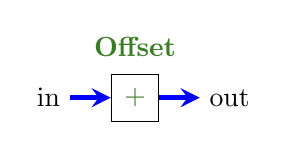
\begin{tikzpicture}
\node[draw, rectangle, minimum size=.6cm] (plus) {{\color{OliveGreen}$+$}};
\node[xshift=-1.1cm] (i) {in};
\node[yshift=+0.65cm] (c) {\textbf{{\color{OliveGreen}Offset}}};
\node[xshift=+1.2cm] (o) {out};
\draw [->,>=stealth,line width=2pt,blue] (i) -- (plus);
\draw [->,>=stealth,line width=2pt,blue] (plus) -- (o);
\end{tikzpicture}  \\

\hline
\includegraphics[width=4.8cm,trim={1cm 9.5cm 1cm 9cm},clip]{figures/splitter.pdf} &Splitter&
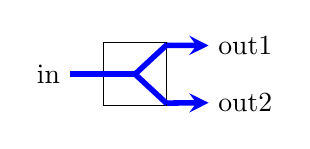
\begin{tikzpicture}
\node[draw, rectangle, minimum size=.8cm] (spl) {};
\node[xshift=-1.1cm] (i) {in};
\node[xshift=+1.4cm,yshift=+0.36cm] (o1) {out1};
\node[xshift=+1.4cm,yshift=-0.36cm] (o2) {out2};
\draw [-,line width=2pt,blue] (spl.west) -- (spl.center);
\draw [-,line width=2pt,blue] (spl.center) -- ([yshift=-0.03cm] spl.north east);
\draw [-,line width=2pt,blue] (spl.center) -- ([yshift=+0.03cm] spl.south east);
\draw [->,>=stealth,line width=2pt,blue] ([yshift=-0.04cm] spl.north east) -- (o1);
\draw [->,>=stealth,line width=2pt,blue] ([yshift=+0.04cm] spl.south east) -- (o2);
\draw [-,>=stealth,line width=2pt,blue] (i) -- (spl);
\end{tikzpicture}   \\

\hline
\includegraphics[width=6cm,trim={6.2cm 11.5cm 4cm 11.5cm},clip]{figures/addsub.pdf} &\hspace*{0.8cm}Combiner.\newline {\color{BlueViolet} Add or subtract signals. The added/subtracted signal is external to the block unlike the add\_const block.}& 
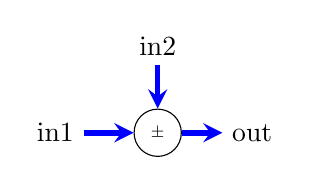
\begin{tikzpicture}
\node[draw, circle, minimum size=.6cm] (plus) {\tiny $\pm$};
\node[xshift=-1.3cm] (i) {in1};
\node[yshift=+1.1cm] (c) {in2};
\node[xshift=+1.2cm] (o) {out};
\draw [->,>=stealth,line width=2pt,blue] (i) -- (plus);
\draw [->,>=stealth,line width=2pt,blue] (plus) -- (o);
\draw [->,>=stealth,line width=2pt,blue] (c) -- (plus);
\end{tikzpicture}  \\

\hline
\includegraphics[width=4.6cm,trim={1cm 9.5cm 1cm 8.5cm},clip]{figures/mixer.pdf} &Mixer, multiplier.& 
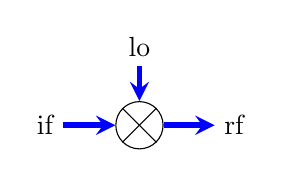
\begin{tikzpicture}
\node [circle, draw ,minimum size=.6cm] (mix) {};
\draw [-] (mix.south west) -- (mix.north east);
\draw [-] (mix.south east) -- (mix.north west);
\node [xshift=-1.2cm] (l) {if};
\node [yshift=+1cm] (u) {lo};
\node [xshift=+1.2cm] (r) {rf};
\draw [->,>=stealth,line width=2pt,blue] (l) -- (mix);
\draw [->,>=stealth,line width=2pt,blue] (u) -- (mix);
\draw [->,>=stealth,line width=2pt,blue] (mix) -- (r);
\end{tikzpicture}  \\

\hline
\includegraphics[width=4.8cm,trim={1cm 9cm 1cm 8cm},clip]{figures/fir.pdf} &\hspace*{0.6cm}Tunable filter.\newline {\color{BlueViolet}FIR with decimation option.}& 
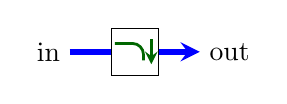
\begin{tikzpicture}
\node[draw, rectangle, minimum size=.6cm] (fir) {};
\node[xshift=-1.1cm] (i) {in};
\node[xshift=+1.2cm] (o) {out};
\draw [-, line width=1pt, color=black!60!green, rounded corners] ([xshift=.05cm,yshift=-.2cm] fir.north west) -| ([xshift=-.2cm,yshift=+.2cm] fir.south east);
\draw [->,>=stealth, line width=1pt, color=black!60!green] ([xshift=-.1cm,yshift=-.15cm] fir.north east) -- ([xshift=-.1cm,yshift=+.15cm] fir.south east);
\draw [line width=2pt,blue] (i) -- (fir);
\draw [->,>=stealth,line width=2pt,blue] (fir) -- (o);
\end{tikzpicture}  \\

\hline
\includegraphics[width=4.5cm,trim={1cm 10cm 1cm 9.5cm},clip]{figures/exp.pdf}\newline
\includegraphics[width=5cm,trim={2cm 11cm 2cm 10.5cm},clip]{figures/shift1.pdf} & {\footnotesize Can be assimilated to $2^m$ amplifiers or attenuators.\newline
{\color{BlueViolet}Are used to adapt the data size between blocks, or to select the range of the numeric signal.\newline
Expander: crop end of word, expand beginning of word. Shift: crop beginning of word, expand end of word.}}& 
\hspace*{0.45cm}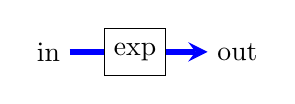
\begin{tikzpicture}
\node[draw, rectangle, minimum size=.6cm] (exp) {exp};
\node[xshift=-1.1cm] (i) {in};
\node[xshift=+1.3cm] (o) {out};
\draw [line width=2pt,blue] (i) -- (exp);
\draw [->,>=stealth,line width=2pt,blue] (exp) -- (o);
\end{tikzpicture} \newline
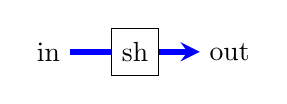
\begin{tikzpicture}
\node[draw, rectangle, minimum size=.6cm] (exp) {sh};
\node[xshift=-1.1cm] (i) {in};
\node[xshift=+1.2cm] (o) {out};
\draw [line width=2pt,blue] (i) -- (exp);
\draw [->,>=stealth,line width=2pt,blue] (exp) -- (o);
\end{tikzpicture} 
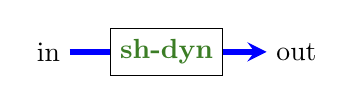
\begin{tikzpicture}
\node[draw, rectangle, minimum size=.6cm] (exp) {\textbf{{\color{OliveGreen}sh-dyn}}};
\node[xshift=-1.5cm] (i) {in};
\node[xshift=+1.65cm] (o) {out};
\draw [line width=2pt,blue] (i) -- (exp);
\draw [->,>=stealth,line width=2pt,blue] (exp) -- (o);
\end{tikzpicture}  \\

\hline

\includegraphics[width=4cm,trim={7.5cm 13.4cm 12.3cm 13.2cm},clip]{figures/switch.pdf} &Switch& 
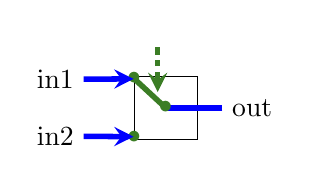
\begin{tikzpicture}	
\usetikzlibrary{arrows}
\node[draw, rectangle, minimum size=.8cm] (spl) {};
\node[xshift=+1.1cm] (i) {out};
\node[yshift=+0.9cm,xshift=-0.1cm] (s) {};
\node[xshift=-1.4cm,yshift=+0.36cm] (o1) {in1};
\node[xshift=-1.4cm,yshift=-0.36cm] (o2) {in2};
\node[OliveGreen, yshift=+0.37cm, xshift=-0.4cm]{$\bullet$};
\node[OliveGreen, yshift=-0.37cm, xshift=-0.4cm]{$\bullet$};
\draw [-,line width=2pt,blue] (spl.east) -- (spl.center);
\draw [-, line width=2pt,OliveGreen] (spl.center) -- ([yshift=-0.03cm] spl.north west);
\draw [<-,>=stealth,line width=2pt,blue] ([yshift=-0.04cm] spl.north west) -- (o1);
\draw [<-,>=stealth,line width=2pt,blue] ([yshift=+0.04cm] spl.south west) -- (o2);
\draw [<-,>=stealth,line width=2pt,OliveGreen,dash dot] ([yshift=+0.2cm,xshift=-0.1cm] spl.center) -- (s);
\draw [-,line width=2pt,blue] (i) -- (spl);
\node[OliveGreen]{$\bullet$};
\end{tikzpicture} \\

\hline

\end{tabular}

\newpage
\vspace*{-1.5cm}
\hspace*{-1cm}
\begin{tabular}{|>{\centering\arraybackslash}m{.3\linewidth} | >{\centering\arraybackslash}m{.3\linewidth} |>{\centering\arraybackslash}m{.3\linewidth}|}
\hline
  & & \\
\textbf{IP} & \textbf{Equivalent RF function {\color{BlueViolet}or numeric function}}&\textbf{ Equivalent scheme with {\color{OliveGreen}tunable entries}} \\
 & & \\
 
 \hline
 \includegraphics[width=3.8cm,trim={2cm 10.5cm 2cm 10cm},clip]{figures/mean.pdf} &\hspace*{0.45cm}Moving average.\newline
 {\color{BlueViolet}Decimation of $2^n$ with averaging: slows the data flow.}
 &
 \begin{tikzpicture}
 \node[draw, rectangle, minimum size=.6cm] (exp) {$\sum~2^n$};
 \draw [->,>=stealth, line width=1pt] ([xshift=-.3cm,yshift=-.15cm] fir.north east) -- ([xshift=-.3cm,yshift=+.15cm] fir.south east);
 \node[xshift=-1.25cm] (i) {in};
 \node[xshift=+1.45cm] (o) {out};
 \draw [line width=2pt,blue] (i) -- (exp);
 \draw [->,>=stealth,line width=2pt,blue] (exp) -- (o);
 \end{tikzpicture}   \\
 
\hline
\includegraphics[width=4.3cm,trim={2cm 9cm 2cm 8.4cm},clip]{figures/delay.pdf} &Tunable delay line ie. cables.   & 
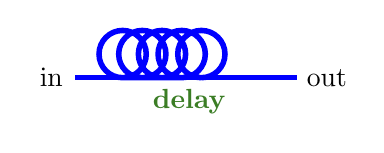
\begin{tikzpicture}
bg
\node[minimum size=.6cm] (i) {in};
\node[xshift=+3.5cm,minimum size=.6cm] (o) {out};
\draw [-,line width=2pt, blue] ([xshift=4em] i.center)+(-0.5cm,0) arc (270:360+270:0.3) -- ([xshift=4em] i.center)+(-0.25cm,0) arc (270:360+270:0.3) -- ([xshift=4em] i.center) arc (270:360+270:0.3) -- ([xshift=4em] i.center)+(.25cm,0) arc (270:360+270:0.3) -- ([xshift=4em] i.center)+(.5cm,0) arc (270:360+270:0.3);
\draw [-,line width=2pt, blue] (i) -- (o);
\node[minimum size=.6cm, yshift=-0.3cm, xshift=+1.75cm] {\textbf{{\color{OliveGreen}delay}}};
\end{tikzpicture}  \\
\hline
 
\hline
\includegraphics[width=4cm,trim={2cm 8.1cm 2cm 7.8cm},clip]{figures/axi2dac.pdf} &Tunable voltage source. \newline{\color{BlueViolet} Controllable states/constants.}&
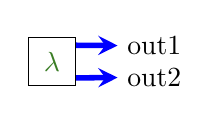
\begin{tikzpicture}
\node[draw, rectangle, minimum size=.6cm] (plus) {\textbf{{\color{OliveGreen}$\lambda$}}};
\node[xshift=+1.3cm, yshift=+0.2cm] (o) {out1};
\node[xshift=+1.3cm, yshift=-0.2cm] (o2) {out2};
\draw [->,>=stealth,line width=2pt,blue] ([yshift=-0.1cm] plus.north east) -- (o);
\draw [->,>=stealth,line width=2pt,blue] ([yshift=+0.1cm] plus.south east) -- (o2);
\end{tikzpicture}  \\

\hline
\includegraphics[width=4.5cm,trim={1cm 6.5cm 1cm 6.4cm},clip]{figures/nco.pdf} 
&\hspace*{0.8cm} DDS \newline {\color{BlueViolet}NCO}& 
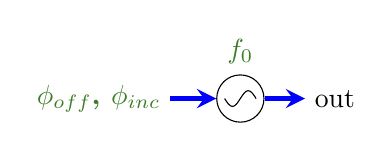
\begin{tikzpicture}	
\node [circle, draw ,minimum size=.6cm] (osc2){};
\node [minimum size=.6cm, yshift=+0.6cm] {\textbf{{\color{OliveGreen}$f_0$}}};
\draw ([xshift=-0.2cm] osc2.center) sin ([xshift=-0.10cm, yshift=-0.10cm] osc2.center) cos (osc2.center) sin ([xshift=0.10cm, yshift=0.10cm] osc2.center) cos ([xshift=0.2cm] osc2.center);
\node [xshift=-1.8cm] (l) {\textbf{{\color{OliveGreen}$\phi_{off}$, $\phi_{inc}$}}};
\node [xshift=+1.2cm] (r) {out};
\draw [->,>=stealth,line width=2pt,blue] (l) -- (osc2);
\draw [->,>=stealth,line width=2pt,blue] (osc2) -- (r);
\end{tikzpicture}  \\

\hline
\includegraphics[width=4cm,trim={7cm 11.6cm 7cm 9.75cm},clip]{figures/pidv3.pdf} &PID&
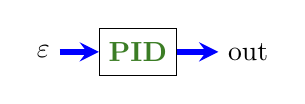
\begin{tikzpicture}
\node[draw, rectangle, minimum size=.6cm] (pid) {\textbf{{\color{OliveGreen}PID}}};
\node[xshift=-1.2cm] (i) {$\varepsilon$};
\node[xshift=+1.4cm] (o) {out};
\draw [->,>=stealth,line width=2pt,blue] (i) -- (pid);
\draw [->,>=stealth,line width=2pt,blue] (pid) -- (o);
\end{tikzpicture}   \\

\hline
\includegraphics[width=3.8cm,trim={1cm 7.45cm 1cm 6.5cm}, clip]{figures/dat2ram.pdf} &Monitoring: oscilloscope, spectrum analyzer...\newline {\color{BlueViolet}Can also be used to process the signal in the CPU. Up to 12 channels.} & 
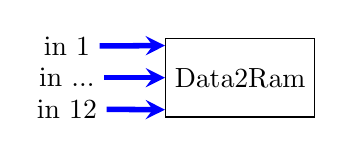
\begin{tikzpicture}
\node[draw, rectangle, minimum size=1cm] (dat) {Data2Ram};
\node[xshift=-2.2cm, yshift=+.4cm] (i1) {in 1};
\node[xshift=-2.2cm, yshift=-.4cm] (i2) {in 12};
\node[xshift=-2.2cm, yshift=0cm] (i) {in ...};
\draw [->,>=stealth,line width=2pt,blue] (i1) -- ([yshift=-.1cm] dat.north west);
\draw [->,>=stealth,line width=2pt,blue] (i2) -- ([yshift=+.1cm]dat.south west);
\draw [->,>=stealth,line width=2pt,blue] (i) -- (dat.west);
\end{tikzpicture}   \\

\hline
\includegraphics[width=4.6cm,trim={7cm 10.55cm 7cm 11.7cm}, clip]{figures/convert} & Split or combine In-phase and Quadrature components.\newline {\color{BlueViolet}Convert $\mathbb{R}$ to $\mathbb{C}$ or $\mathbb{C}$ to $\mathbb{R}$.} & 
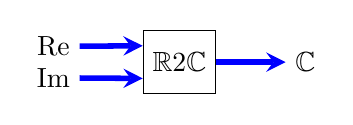
\begin{tikzpicture}
\node[draw, rectangle, minimum size=0.8cm] (dat) {$\mathbb{R}$2$\mathbb{C}$};
\node[xshift=-1.6cm, yshift=+.2cm] (i1) {Re};
\node[xshift=-1.6cm, yshift=-.2cm] (i2) {Im};
\node[xshift=+1.6cm, yshift=0cm] (i) {$\mathbb{C}$};
\draw [->,>=stealth,line width=2pt,blue] (i1) -- ([yshift=-.2cm] dat.north west);
\draw [->,>=stealth,line width=2pt,blue] (i2) -- ([yshift=+.2cm]dat.south west);
\draw [->,>=stealth,line width=2pt,blue] (dat.east) -- (i);
\end{tikzpicture} 
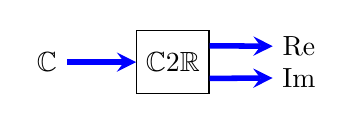
\begin{tikzpicture}
\node[draw, rectangle, minimum size=0.8cm] (dat) {$\mathbb{C}$2$\mathbb{R}$};
\node[xshift=+1.6cm, yshift=+.2cm] (i1) {Re};
\node[xshift=+1.6cm, yshift=-.2cm] (i2) {Im};
\node[xshift=-1.6cm, yshift=0cm] (i) {$\mathbb{C}$};
\draw [<-,>=stealth,line width=2pt,blue] (i1) -- ([yshift=-.2cm] dat.north east);
\draw [<-,>=stealth,line width=2pt,blue] (i2) -- ([yshift=+.2cm]dat.south east);
\draw [<-,>=stealth,line width=2pt,blue] (dat.west) -- (i);
\end{tikzpicture}  \\

\hline
\end{tabular}

\section{Webserver}\label{sect:webserver}

The tunable parameters of the IPs are controlled through C coded functions, visible in the /oscimpDigital/lib/my\_lib.h library files. Example of functions with a generic driver "fpgagen":

\vspace{-0.2cm}
\begin{lstlisting}[language=C]
fpgagen_send_conf(char *filename, int reg, int value); 
fpgagen_recv_conf(char *filename, int reg, int *value);
\end{lstlisting}

\hspace{1cm}

Those functions can be implemented in a graphic interface to constitute a user friendly control of the IPs. Here we show an example of webserver using RemI\footnote{Download and Faq : https://www.remigui.com/}, a cross platform remote gui for python. The wrapper liboscimp\_fpga.py makes the intermediary between the webserver and the libraries. It takes the following form:

\vspace{-0.2cm}
\begin{lstlisting}[language=Python]
import ctypes
from ctypes import *
lib = ctypes.CDLL('/usr/lib/liboscimp_fpga.so')

def fpgagen_send_conf(filename, reg, value):
		file = ctypes.create_string_buffer(str.encode(filename))
		my_val = int(value)
		lib.fpgagen_send_conf(file, reg, my_val)

def fpgagen_recv_conf(filename, reg):
		file = ctypes.create_string_buffer(str.encode(filename))
		my_val = c_int()
		ret_val = lib.fpgagen_recv_conf(file, reg, byref(my_val))
		return (ret_val, my_val.value)
\end{lstlisting}

\hspace{1cm}

Then the example of functions implemented in the webserver to configure the IPs is:

\vspace{-0.2cm}
\begin{lstlisting}[language=Python]
import liboscimp_fpga
liboscimp_fpga.fpgagen_send_conf("/dev/my_file", my_reg, my_value)
\end{lstlisting}

\hspace{1cm}

In the webserver, values sent to the IPs can either take the form of slider, a spinbox, a checkbox, a button... In our case, a simple actuator will be represented by a checkbox, and any other controllable value by both a slider and a spinbox. The structure of the webserver is as follows:

\vspace{-0.2cm}
\begin{lstlisting}[language=Python]
#!/usr/bin/env python

import liboscimp_fpga
import ctypes
import remi.gui as gui
from remi import start, App

class MyApp(App):
		def __init__(self, *args):
				super(MyApp, self).__init__(*args)

		def main(self):
				self.w = gui.VBox()
				
				#Create the slider and the spinbox, whose value is restricted to -8192 to 8191 (no overflow)
				self.hbox_MY_VALUE = gui.HBox(margin="10px")
				self.lb_MY_VALUE = gui.Label("/dev/MY_VALUE_FILE", width="20%", margin="50px")
				self.sd_MY_VALUE = gui.Slider(0, -8192, 8191, 1, width="60%", margin="10px")
				self.sd_MY_VALUE.set_oninput_listener(self.sd_MY_VALUE_changed)
				self.sb_MY_VALUE = gui.SpinBox(0, -8192, 8191, 1, width="20%", margin="10px")
				self.sb_MY_VALUE.set_on_change_listener(self.sb_MY_VALUE_changed)
				self.sd_MY_VALUE_changed(self.sd_MY_VALUE, self.sd_MY_VALUE.get_value())
				self.hbox_MY_VALUE.append(self.lb_MY_VALUE)
				self.hbox_MY_VALUE.append(self.sd_MY_VALUE)
				self.hbox_MY_VALUE.append(self.sb_MY_VALUE)
				self.w.append(self.hbox_MY_VALUE)

				#Create the checkbox
				self.hbox_MY_ACTUATOR = gui.HBox(margin="10px")
				self.lb_MY_ACTUATOR = gui.Label("/dev/MY_ACTUATOR_FILE", width="20%", margin="50px")
				self.cb_MY_ACTUATOR = gui.CheckBox(True, width="5%", margin="10px")
				self.cb_MY_ACTUATOR.set_on_change_listener(self.cb_MY_ACTUATOR_changed)
				self.hbox_MY_ACTUATOR.append(self.lb_MY_ACTUATOR)
				self.hbox_MY_ACTUATOR.append(self.cb_MY_ACTUATOR)
				self.w.append(self.hbox_MY_ACTUATOR)

				return self.w
		
		#Function called by the slider
		def sd_MY_VALUE_changed(self, widget, value):
				print("/dev/MY_VALUE_FILE", MY_REG, int(value))
				liboscimp_fpga.fpgagen_send_conf("/dev/MY_VALUE_FILE", MY_REG, int(value))
				self.sb_MY_VALUE.set_value(int(value))

		#Function called by the spinbox
		def sb_MY_VALUE_changed(self, widget, value):
				print("/dev/MY_VALUE_FILE", MY_REG, int(value))
				liboscimp_fpga.fpgagen_send_conf("/dev/MY_VALUE_FILE", MY_REG, int(value))
				self.sd_MY_VALUE.set_value(int(float(value)))
				
		#Function called by the checkbox
		def sb_MY_ACTUATOR_changed(self, widget, value):
				print("/dev/MY_ACTUATOR_FILE", MY_REG, int(value))
				liboscimp_fpga.fpgagen_send_conf("/dev/MY_ACTUATOR_FILE", MY_REG2, int(value))
				self.sd_adc1_offset.set_value(int(float(value)))

#Launch oh the webserver on the local machine
start(MyApp, address="0.0.0.0", port=80, title="My_super_webserver")
\end{lstlisting}

Preview of the webserver created:

\begin{figure}[h!tb]
	\begin{center}
		\includegraphics[width=15cm]{webserver/Super_webserver.png}
		\caption{Example of webserver with MY\_VALUE\_FILE represented by a slider and a spinbox, and MY\_ACTUATOR\_FILE represented by a checkbox.}
		\label{fig:superwebserver}
	\end{center}
\end{figure}

Here the generic driver fpgagen is used as an example, however the use of a different driver can lead to various requirements: arguments, data type, or several functions. Some specific cases will be treated in the next sections. In the other cases, refer to the /oscimpDigital/lib/my\_lib.h library files, or the oscimpDigital documentation: \href{[https://github.com/oscimp/oscimpDigital/tree/master/doc]}{https://github.com/oscimp/oscimpDigital/tree/master/doc}
\newline \newline
A webserver generator is available in the /oscimpDigital/app/tools/webserver\_generator repository, and build a standard webserver using the same My\_super\_design.xml file than the one used by the module generator :

 \begin{lstlisting}[language=bash]
./webserver_generator.py My_super_design.xml
 \end{lstlisting}

\section{Double voltage source}

A double tunable voltage source can be set up si using the axi\_to\_dac IP. However it's only one of the many functions that can be imagined with this IP. 
\newline See \href{[https://github.com/oscimp/oscimpDigital/blob/master/doc/IP/axi_to_dac.md]}{https://github.com/oscimp/oscimpDigital/blob/master/doc/IP/axi\_to\_dac.md}.
The block diagram is as follows :

\begin{figure}[h!tb]
	\begin{center}
		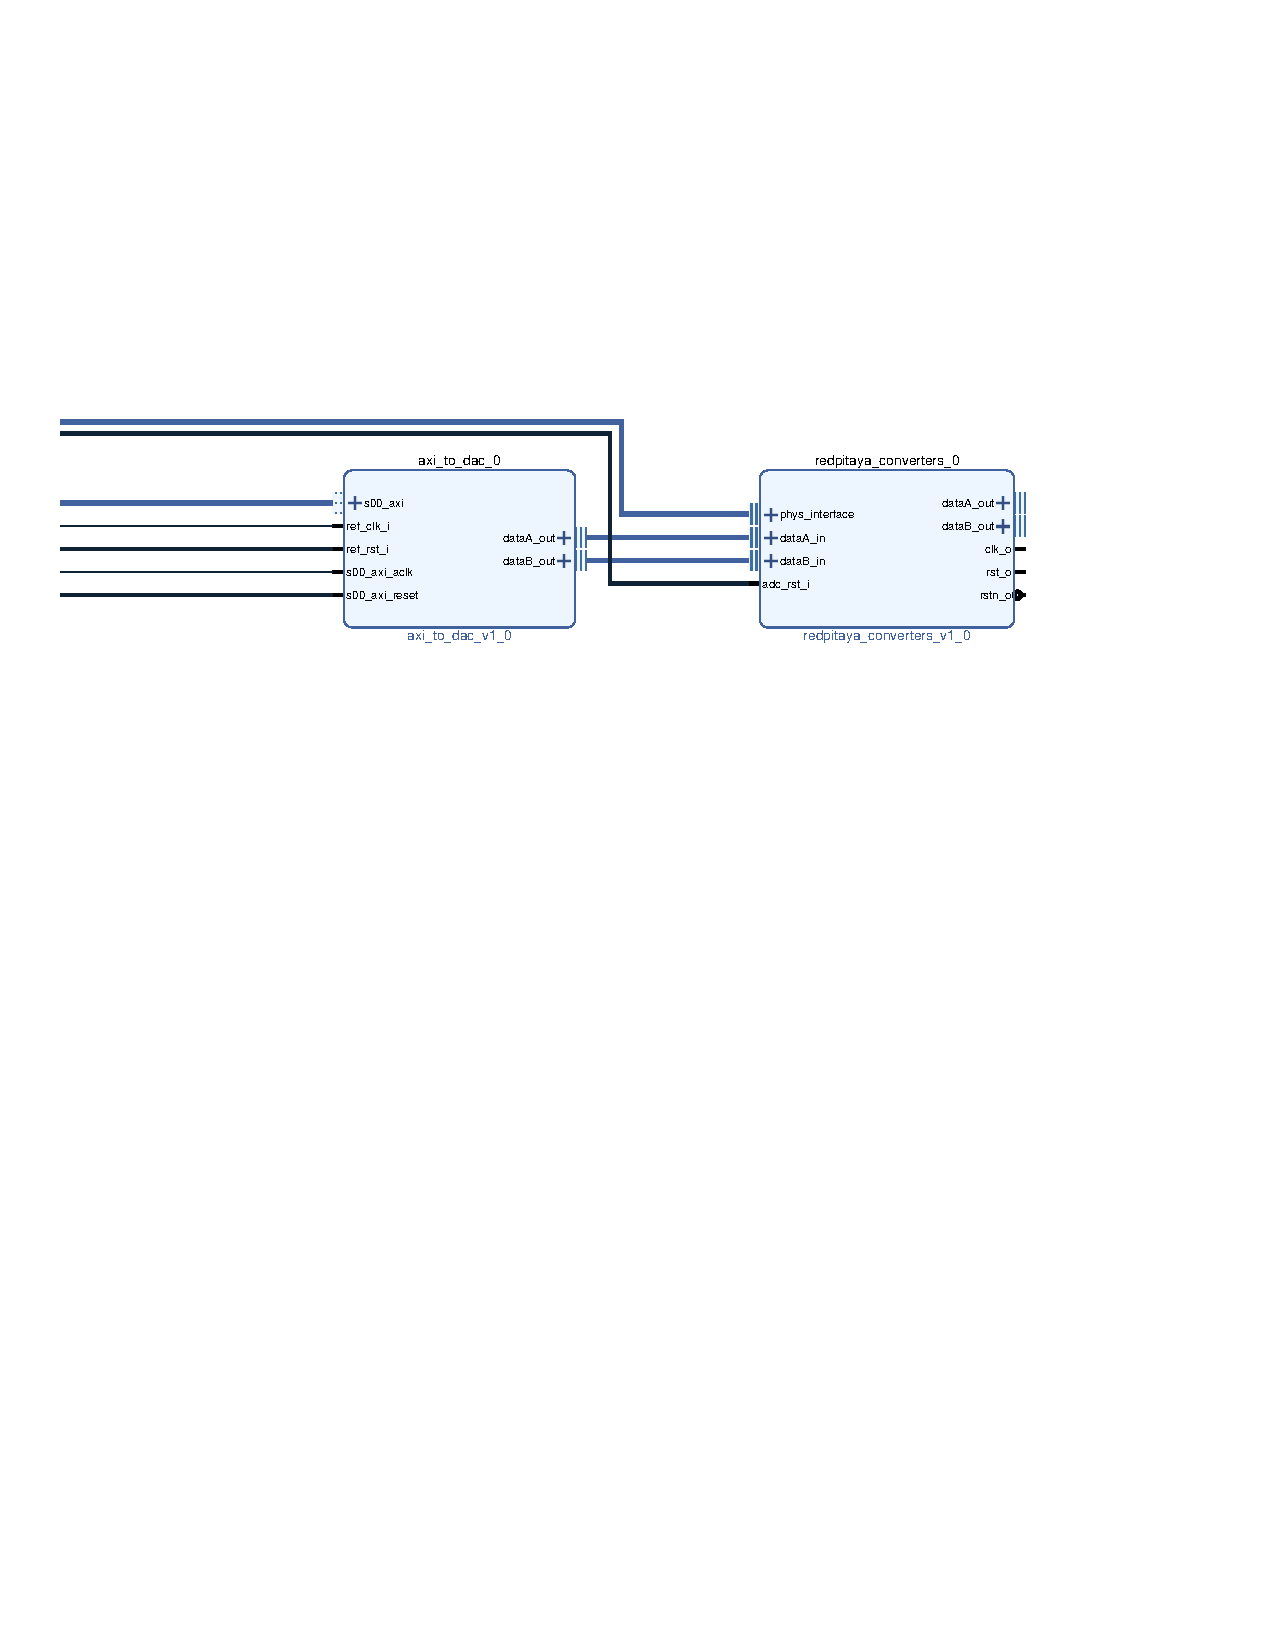
\includegraphics[width=12cm,trim={4.5cm 16cm 3.5cm 7cm}, clip]{figures/GeneTension.pdf}
		\caption{Part of the block diagram for the tunable voltage source.}
		\label{fig:geneTension}
	\end{center}
\end{figure}
\vspace{3cm}
In this configuration and with data on $14~bits$, all the parameters of the axi\_to\_dac block keep their default value. The tuning of the output is performed with the webserver (see section \ref{sect:webserver}). With the Redpitaya board, the maximum voltage is $\pm 1~V$ per output.
\vspace{1cm}
\section{Double DDS}

The schematic configuration of the double DDS we propose here is shown below: 
\vspace{0.5cm}
\begin{center}
	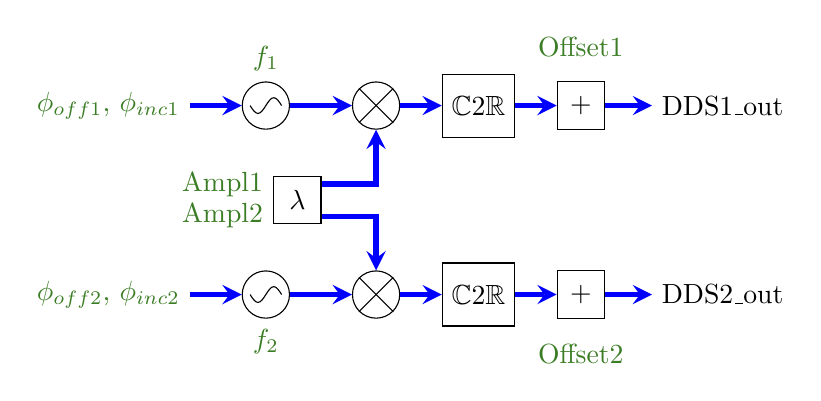
\begin{tikzpicture}	
\node[draw, rectangle, minimum size=.6cm] (plus) {$\lambda$};
\node[left of=plus, xshift=+0.05cm, yshift=+0.2cm] {{\color{OliveGreen}Ampl1}};
\node[left of=plus, xshift=+0.05cm, yshift=-0.2cm] {{\color{OliveGreen}Ampl2}};

\node [circle, draw ,minimum size=.6cm, xshift=-0.4cm, yshift=+0.2cm, above of=plus] (osc2){};
\node[above of=osc2, yshift=-0.4cm] {{\color{OliveGreen}$f_1$}};
\node [circle, draw ,minimum size=.6cm, xshift=-0.4cm, yshift=-0.2cm, below of=plus] (osc1){};
\node[below of=osc1, yshift=+0.4cm] {{\color{OliveGreen}$f_2$}};
\draw ([xshift=-0.2cm] osc2.center) sin ([xshift=-0.10cm, yshift=-0.10cm] osc2.center) cos (osc2.center) sin ([xshift=0.10cm, yshift=0.10cm] osc2.center) cos ([xshift=0.2cm] osc2.center);
\draw ([xshift=-0.2cm] osc1.center) sin ([xshift=-0.10cm, yshift=-0.10cm] osc1.center) cos (osc1.center) sin ([xshift=0.10cm, yshift=0.10cm] osc1.center) cos ([xshift=0.2cm] osc1.center);
\node [xshift=-1cm, left of=osc2] (l1) {{\color{OliveGreen}$\phi_{off1}$, $\phi_{inc1}$}};
\draw [->,>=stealth,line width=2pt,blue] (l1) -- (osc2);
\node [xshift=-1cm, left of=osc1] (l2) {{\color{OliveGreen}$\phi_{off2}$, $\phi_{inc2}$}};
\draw [->,>=stealth,line width=2pt,blue] (l2) -- (osc1);


\node [circle, draw ,minimum size=.6cm, xshift=0.4cm, right of= osc1] (mix1) {};
\draw [-] (mix1.south west) -- (mix1.north east);
\draw [-] (mix1.south east) -- (mix1.north west);
\node [circle, draw ,minimum size=.6cm, xshift=0.4cm, right of= osc2] (mix2) {};
\draw [-] (mix2.south west) -- (mix2.north east);
\draw [-] (mix2.south east) -- (mix2.north west);

\draw [->,>=stealth,line width=2pt,blue] ([yshift=-0.1cm] plus.north east) -| (mix2);
\draw [->,>=stealth,line width=2pt,blue] ([yshift=+0.1cm] plus.south east) -| (mix1);

\draw [->,>=stealth,line width=2pt,blue] (osc1) -- (mix1);
\draw [->,>=stealth,line width=2pt,blue] (osc2) -- (mix2);

\node[draw, rectangle, minimum size=0.8cm, right of=mix1, xshift=0.3cm] (dat1) {$\mathbb{C}$2$\mathbb{R}$};
\node[draw, rectangle, minimum size=0.8cm, right of=mix2, xshift=0.3cm] (dat2) {$\mathbb{C}$2$\mathbb{R}$};

\draw [->,>=stealth,line width=2pt,blue] (mix1) -- (dat1);
\draw [->,>=stealth,line width=2pt,blue] (mix2) -- (dat2);

\node[draw, rectangle, minimum size=.6cm, xshift=0.3cm, right of=dat1] (plu) {$+$};
\node[yshift=0.25cm, below of=plu] (c1) {{\color{OliveGreen}Offset2}};
\node[xshift=0.8cm, right of=plu] (o1) {DDS2\_out};
\draw [->,>=stealth,line width=2pt,blue] (plu) -- (o1);

\node[draw, rectangle, minimum size=.6cm, xshift=0.3cm, right of=dat2] (plu2) {$+$};
\node[yshift=-0.25cm, above of=plu2] (c2) {{\color{OliveGreen}Offset1}};
\node[xshift=0.8cm, right of=plu2] (o2) {DDS1\_out};
\draw [->,>=stealth,line width=2pt,blue] (plu2) -- (o2);

\draw [->,>=stealth,line width=2pt,blue] (dat1) -- (plu);
\draw [->,>=stealth,line width=2pt,blue] (dat2) -- (plu2);
\end{tikzpicture} 
\end{center} 
\vspace{0.5cm}
It corresponds to two DDS with adjustable frequency, amplitude, output offset, and referenced on the same clock. Frequency/phase and amplitude modulation are not represented here, but can be added using sections \ref{sect:AM1} and \ref{sect:FMPM}. The block diagram associated with this scheme is as follows:

\begin{figure}[h!tb]
	\begin{center}
		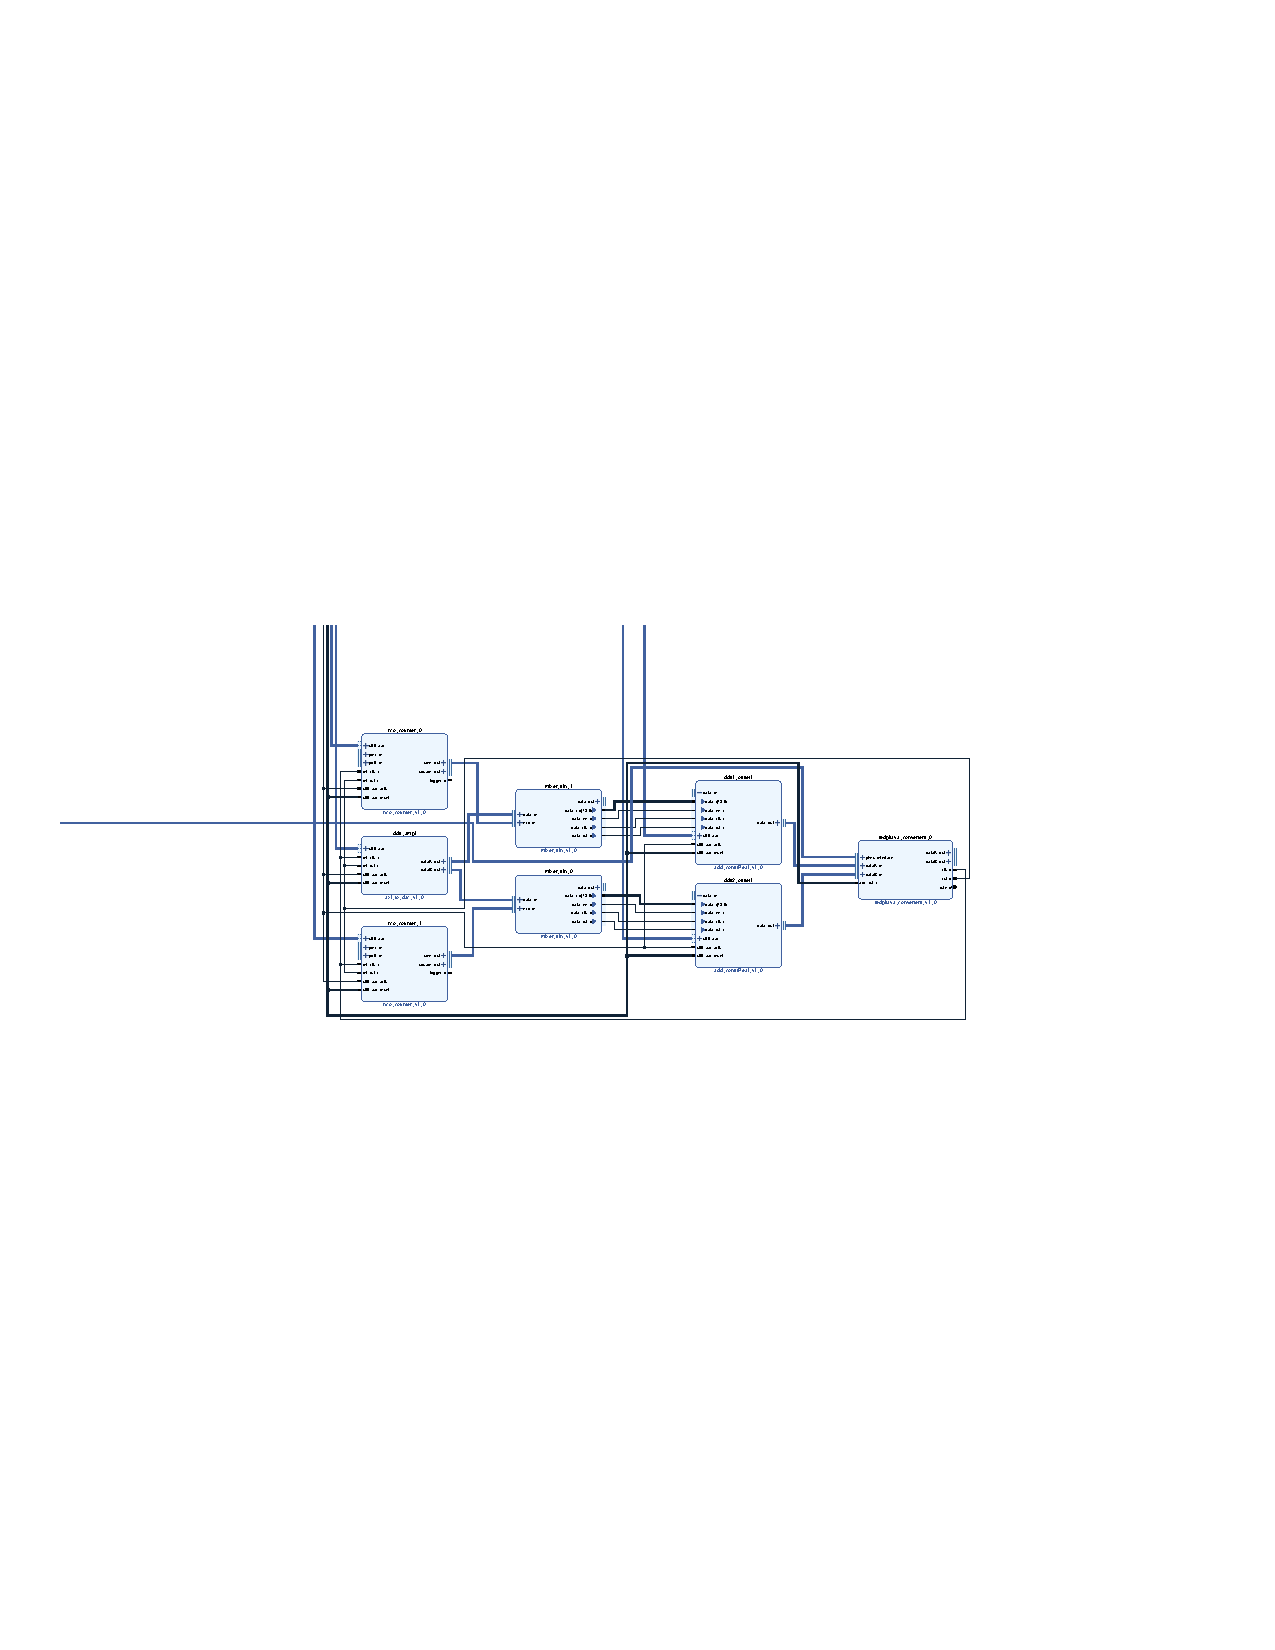
\includegraphics[width=16cm,trim={1cm 5.5cm 1cm 11cm}, clip]{figures/doubleDDS.pdf}
		\caption{Part of the block diagram for the double DDS.}
		\label{fig:doubleDDS}
	\end{center}
\end{figure}

\newpage
\subsection{IP configuration}
\vspace{0.5cm}
The IPs configuration may change depending on the board/application, however in this example we used the following configurations:
\begin{center}
	\begin{tabular}{|>{\centering\arraybackslash}m{.3\linewidth} | >{\centering\arraybackslash}m{.3\linewidth} |}
\hline
IP & Configuration \\
\hline
 & Counter size: $40~bits$\\ nco\_counter\_1/2 &Data size: $16~bits$\\ &Lut size: $12~bits$ \\
\hline
dds\_ampl&Data size: $14~bits$ \\
\hline
mixer\_sin\_1/2&Data in/out size: $14~bits$ \newline Nco\_size: $16~bits$ \\
\hline
dds1/2\_offset&Data in size: $14~bits$\newline Data out size: $14~bits$\newline Signed \\
\hline
convert$\mathbb{C}$to$\mathbb{R}$\_1/2&Data size: $14~bits$\\
\hline
\end{tabular}
\end{center}
\vspace{0.1cm}
\subsection{Webserver configuration}\label{subsec:doubleDDSws}

For the DDS offset and amplitude blocks we only use one value to be controlled, ie. one slider/spinbox. However the NCO block offers several options as the phase offset and increment can be internal or external to the block. Therefore we keep a default construction for the NCO in the webserver, including all these possibilities: 
\begin{itemize}
	\setlength\itemsep{-0.1cm}
	\item 1$^{st}$ slider+spinbox: the frequency control, up to the half clock frequency (Hz)
	\item 2$^{nd}$ slider+spinbox: the phase offset control
	\item pinc checkbox: internal or external phase increment
	\item poff checkbox: internal or external phase increment
\end{itemize} 

In the present case there is no external connections for the frequency and phase increments, thus the pinc and poff checkbox will remain checked. A preview of the webserver for the double DDS design is given in fig.\ref{fig:webdoubleDDS}.

\begin{figure}[!h!tb]
	\begin{center}
		\includegraphics[width=14cm]{webserver/2019-10-14-143651_927x541_scrot.png}
		\caption{Screenshot of the double DDS webserver.}
		\label{fig:webdoubleDDS}
	\end{center}
\end{figure}

\vspace{0cm}

\subsection{Expected output}

We show in fig.\ref{fig:doubleDDSok} an example of twe signals generated. \newline 
Ch1: $f_0=30~MHz$, $dds1\_ampl=8191~arb.~unit$, $dds1\_offset=0~arb.~unit$, \newline $\phi_{off1}=0~arb.~unit$.\newline
Ch2: $f_0=45~MHz$, $dds2\_ampl=3000~arb.~unit$, $dds2\_offset=5000~arb.~unit$, \newline $\phi_{off2}=0~arb.~unit$.

\begin{figure}[h!tb]
	\begin{center}
		\includegraphics[width=14cm]{scope/doubleDDSok.pdf}
		\caption{Expected output.}
		\label{fig:doubleDDSok}
	\end{center}
\end{figure}

With an internal phase increment, the output signals are generated with an arbitrary phase. This phase can be adjusted according to the intended application, using the phase offset slider, as represented in fig.\ref{fig:doubleDDSphase}:

\begin{figure}[h!tb]
	\begin{center}
		\includegraphics[width=14cm]{scope/doubleDDSokPhi.pdf}
		\caption{Phase offset.}
		\label{fig:doubleDDSphase}
	\end{center}
\end{figure}

\vspace{-1cm}
\subsection{Unexpected output}\label{subsect:doubleDDSpasOk}

In fig.\ref{fig:doubleDDSpasOk} the Ch1 signal is the same, but there is an overflow in Ch2 due to the sum of $dds1\_ampl$ and $dds1\_offset$. \newline
Ch2: $f_0=45~MHz$, $dds2\_ampl=8191~arb.~unit$, $dds2\_offset=8191~arb.~unit$, \newline $\phi_{off2}=0~arb.~unit$.

\begin{figure}[!h!tb]
	\begin{center}
		\includegraphics[width=14cm]{scope/doubleDDSpasOk.pdf}
		\caption{Unexpected output due to overflow in ch2.}
		\label{fig:doubleDDSpasOk}
	\end{center}
\end{figure}
Solution: decrease either $dds1\_ampl$ or $dds1\_offset$, such as ${dds1\_ampl + dds1\_offset < 8191}$.

\section{Amplitude modulation}\label{sect:AM1}

An amplitude modulation can be performed easily, in the same way as with RF components:

\begin{center}
	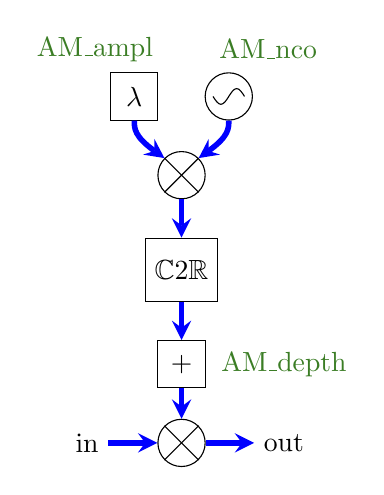
\begin{tikzpicture}	
	\node[draw, rectangle, minimum size=.6cm] (plus) {$\lambda$};
	\node[above of=plus, yshift=-0.4cm, xshift=-0.5cm] {{\color{OliveGreen}AM\_ampl}};
	\node [circle, draw ,minimum size=.6cm, xshift=+0.6cm, below of=plus] (mix1) {};
	\draw [-] (mix1.south west) -- (mix1.north east);
	\draw [-] (mix1.south east) -- (mix1.north west);
	
	\node[draw, rectangle, minimum size=0.8cm, below of=mix1, yshift=-0.2cm] (dat) {$\mathbb{C}$2$\mathbb{R}$};
	\node[draw, rectangle, minimum size=.6cm, below of=dat, yshift=-0.2cm] (plu) {+};
	\node[right of=plu, xshift=+0.3cm] {{\color{OliveGreen}AM\_depth}};
	\node [circle, draw ,minimum size=.6cm, below of=plu] (mix2) {};
	\draw [-] (mix2.south west) -- (mix2.north east);
	\draw [-] (mix2.south east) -- (mix2.north west);
	
	\node [circle, draw ,minimum size=.6cm, above of=mix1, xshift=0.6cm] (osc1){};
	\node[above of=osc1, yshift=-0.4cm, xshift=+0.5cm] {{\color{OliveGreen}AM\_nco}};
	\draw ([xshift=-0.2cm] osc1.center) sin ([xshift=-0.10cm, yshift=-0.10cm] osc1.center) cos (osc1.center) sin ([xshift=0.10cm, yshift=0.10cm] osc1.center) cos ([xshift=0.2cm] osc1.center);
	
	
	\node[xshift=0.8cm, left of=mix2, xshift=-1cm] (i1) {in};
	\node[xshift=0.8cm, right of=mix2, xshift=-0.5cm] (o1) {out};
	\draw [->,>=stealth,line width=2pt,blue] (mix2) -- (o1);
	\draw [->,>=stealth,line width=2pt,blue] (i1) -- (mix2);
	\draw [->,>=stealth,line width=2pt,blue] (plu) -- (mix2);
	\draw [->,>=stealth,line width=2pt,blue] (mix1) -- (dat);
	\draw [->,>=stealth,line width=2pt,blue] (dat) -- (plu);
	
	\draw [->, >=stealth, line width=2pt, blue] (plus.south) .. controls ([xshift=0cm, yshift=-0.1cm] plus.south) and ([xshift=0em, yshift=-0.2cm] plus.south) ..(mix1.north west);
	
	\draw [->, >=stealth, line width=2pt, blue] (osc1.south) .. controls ([xshift=0cm, yshift=-0.1cm] osc1.south) and ([xshift=0em, yshift=-0.2cm] osc1.south) ..(mix1.north east);
	\end{tikzpicture} 
\end{center}
\vspace{-0.3cm}
This scheme is equivalent to the expression of the amplitude modulation:
\begin{center}
	 ${y(t)=[1 + h~cos(\omega_m t)]z(t)}$\newline

	 $\Rightarrow{out=[1 + \frac{AM\_ampl}{AM\_depth} AM\_nco]~AM\_depth\times in}$
\end{center}

Then the modulation depth is $h=\frac{AM\_ampl}{AM\_depth}$. Thereafter:
\vspace{-0.1cm}
\begin{itemize}
	\setlength\itemsep{-0.2cm}
	\item $h=0$ with $AM\_ampl=0$ 
	\item $h=0.5$ with $AM\_ampl=4096~arb.~unit$ and $AM\_depth=8191~arb.~unit$
	\item $h=1$ with $AM\_ampl=8191~arb.~unit$ and $AM\_depth=8191~arb.~unit$
	\item $h=2$ with $AM\_ampl=8191~arb.~unit$ and $AM\_depth=4096~arb.~unit$
\end{itemize}The block diagram corresponding to this scheme is as follows:\newpage

\begin{figure}[h!tb]
	\begin{center}
		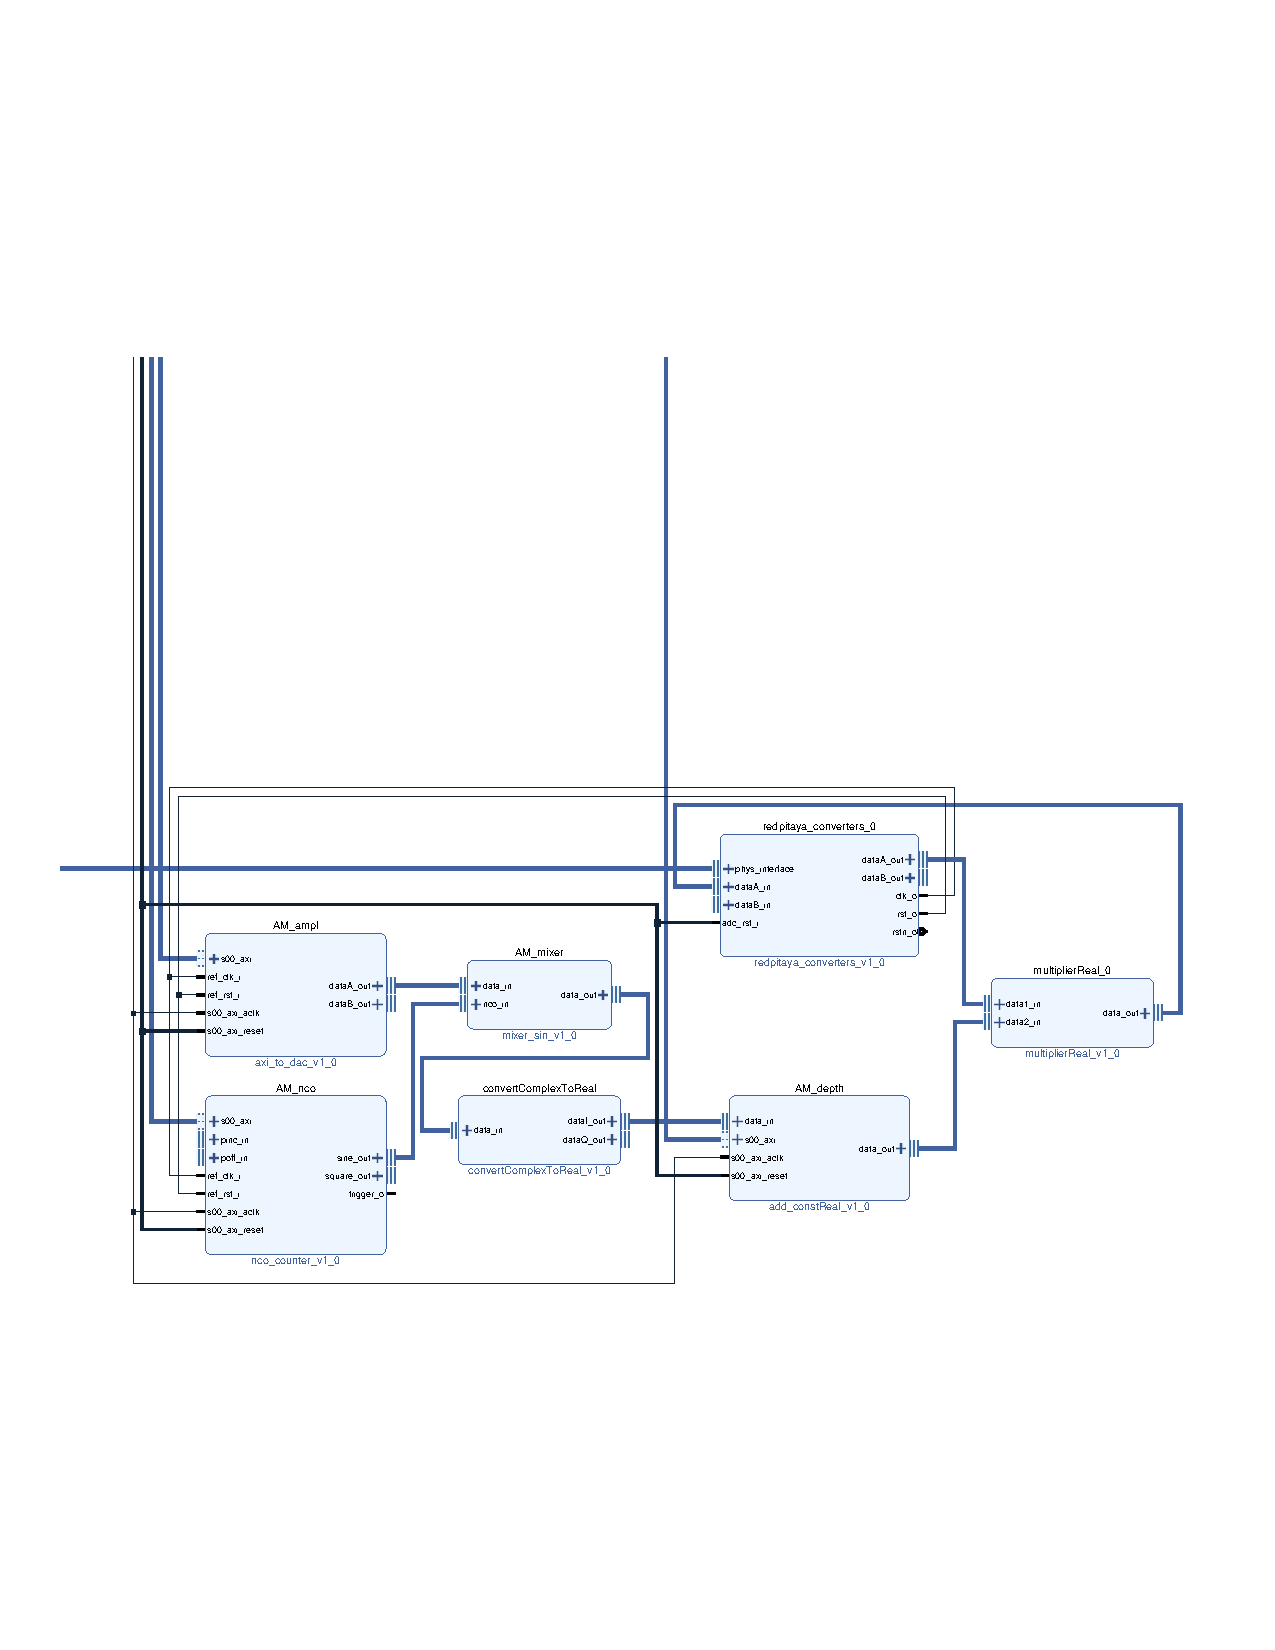
\includegraphics[width=14cm,trim={1.8cm 6cm 1cm 13cm}, clip]{design/mod_ampl1.pdf}
		\caption{Part of the block diagram for this amplitude modulation.}
		\label{fig:mod_ampl1}
	\end{center}
\end{figure}

In this block diagram the input and output are connected to the converter blocks to make an example with external signal. However this principle can be included to other applications, such as the double dds design to add an amplitude modulation option to the generated signals.
\vspace{-0.3cm}
\subsection{IP configuration}
\vspace{-0cm}
IPs configuration in this example:
\begin{center}
	\begin{tabular}{|>{\centering\arraybackslash}m{.3\linewidth} | >{\centering\arraybackslash}m{.3\linewidth} |}
		\hline
		IP & Configuration \\
		\hline
		& Counter size: $40~bits$\\ AMo\_nco &Data size: $16~bits$\\ &Lut size: $12~bits$ \\
		\hline
		AM\_ampl&Data size: $16~bits$ \\
		\hline
		AM\_mixer&Data in/out size: $16~bits$ \newline Nco\_size: $16~bits$ \\
		\hdashline
		multiplierReal&Input data1 size: $14~bits$ \newline Input data2 size: $16~bits$\newline Output data size: $14~bits$ \\
		\hline
		& Data in size: $16~bits$\\AM\_depth & Data out size: $16~bits$\\ &Format: Signed \\
		\hline
		convert$\mathbb{C}$to$\mathbb{R}$\_1&Data size: $16~bits$\\
		\hline
	\end{tabular}
\end{center}
\vspace{-0.2cm}
\subsection{Webserver configuration}

Here the webserver configuration is similar to the double dds one. In case refer to subsection \ref{subsec:doubleDDSws}. preview of the amplitude modulation part of the webserver, with the mod\_nco controlling the modulation frequency, and mod\_ampl controlling its amplitude:

\begin{figure}[!h!tb]
	\begin{center}
		\includegraphics[width=14cm]{webserver/AM_V1.png}
		\caption{Screenshot of the amplitude modulation part of the webserver.}
		\label{fig:amplModWsv1}
	\end{center}
\end{figure}


\subsection{Expected output}

To make a small preview of the expected behavior of the amplitude modulation, we will present the cases $h=0.5$, $h=1$, and the surmodulation $h=2$. We use at the input a sine signal of $50~MHz$ and $0~dBm$. The modulating signal is set to $500~kHz$.\newline

\underline{Input and output with $h=0.5$}

\begin{figure}[!h!tb]
	\begin{center}
		\includegraphics[width=14cm]{scope/Mod_amplOkV1h05.pdf}
		\caption{Expected behavior for $h=0.5$.}
		\label{fig:ampleModV11}
	\end{center}
\end{figure}

\underline{Output with $h=1$}

\begin{figure}[!h!tb]
	\begin{center}
		\includegraphics[width=14cm]{scope/Mod_amplOkV1h10.pdf}
		\caption{Expected behavior for $h=1$.}
		\label{fig:ampleModV12}
	\end{center}
\end{figure}
\newpage
\underline{Output with $h=2$ (overmodulation)}

\begin{figure}[!h!tb]
	\begin{center}
		\includegraphics[width=14cm]{scope/Mod_amplOkV1h20.pdf}
		\caption{Expected behavior for $h=2$: overmodulation.}
		\label{fig:ampleModV13}
	\end{center}
\end{figure}

\subsection{Unexpected output}

Although the following case is not due to the numerical aspect of the amplitude modulation presented here, it can be seen as an unexpected output:

\begin{figure}[!h!tb]
	\begin{center}
		\includegraphics[width=14cm]{scope/Mod_amplPasOkV1.pdf}
		\caption{Case of a carrier frequency below the input signal frequency.}
		\label{fig:ampleModV14}
	\end{center}
\end{figure}

This kind of shape is due to a carrier frequency below the input signal frequency. 
 
\section{Sine perturbation of a signal}\label{sect:AM2}
\vspace{0.5cm}
A way to study the response of a system is to apply a perturbation to this system. Most of the time, the perturbations take the form of steps applied to the input signal of the system by adding to it a square signal. In the case of optical oscillators, the working point of the system, i.e. the resonant frequency, can be determined by making a frequency scan of the system. This scan takes the form of a sine perturbation of the system. In this section, we show the example of a sine perturbation to a signal. The scheme used is quite similar to the amplitude modulation:
\vspace{0.5cm}
\begin{center}
	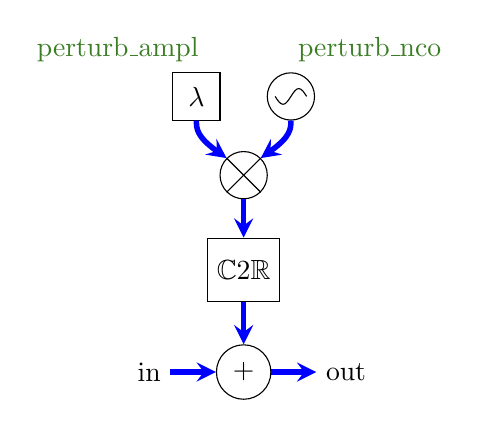
\begin{tikzpicture}	
	\node[draw, rectangle, minimum size=.6cm] (plus) {$\lambda$};
	\node[above of=plus, yshift=-0.4cm, xshift=-1cm] {{\color{OliveGreen}perturb\_ampl}};
	\node [circle, draw ,minimum size=.6cm, xshift=+0.6cm, below of=plus] (mix1) {};
	\draw [-] (mix1.south west) -- (mix1.north east);
	\draw [-] (mix1.south east) -- (mix1.north west);
	\node[draw, rectangle, minimum size=0.8cm, yshift=-0.2cm, below of=mix1] (c2r) {$\mathbb{C}$2$\mathbb{R}$};
	\node [circle, draw ,minimum size=.6cm, yshift=-0.3cm, below of=c2r] (mix2) {+};
	
	\node [circle, draw ,minimum size=.6cm, above of=mix1, xshift=0.6cm] (osc1){};
	\node[above of=osc1, yshift=-0.4cm, xshift=+1cm] {{\color{OliveGreen}perturb\_nco}};
	\draw ([xshift=-0.2cm] osc1.center) sin ([xshift=-0.10cm, yshift=-0.10cm] osc1.center) cos (osc1.center) sin ([xshift=0.10cm, yshift=0.10cm] osc1.center) cos ([xshift=0.2cm] osc1.center);
	
	\node[xshift=0.8cm, left of=mix2, xshift=-1cm] (i1) {in};
	\node[xshift=0.8cm, right of=mix2, xshift=-0.5cm] (o1) {out};
	\draw [->,>=stealth,line width=2pt,blue] (mix2) -- (o1);
	\draw [->,>=stealth,line width=2pt,blue] (i1) -- (mix2);
	\draw [->,>=stealth,line width=2pt,blue] (mix1) -- (c2r);
	\draw [->,>=stealth,line width=2pt,blue] (c2r) -- (mix2);
	
	\draw [->, >=stealth, line width=2pt, blue] (plus.south) .. controls ([xshift=0cm, yshift=-0.1cm] plus.south) and ([xshift=0em, yshift=-0.2cm] plus.south) ..(mix1.north west);
	
	\draw [->, >=stealth, line width=2pt, blue] (osc1.south) .. controls ([xshift=0cm, yshift=-0.1cm] osc1.south) and ([xshift=0em, yshift=-0.2cm] osc1.south) ..(mix1.north east);
	\end{tikzpicture} 
\end{center}

The block diagram corresponding to this scheme is as follows:

\begin{figure}[h!tb]
	\begin{center}
		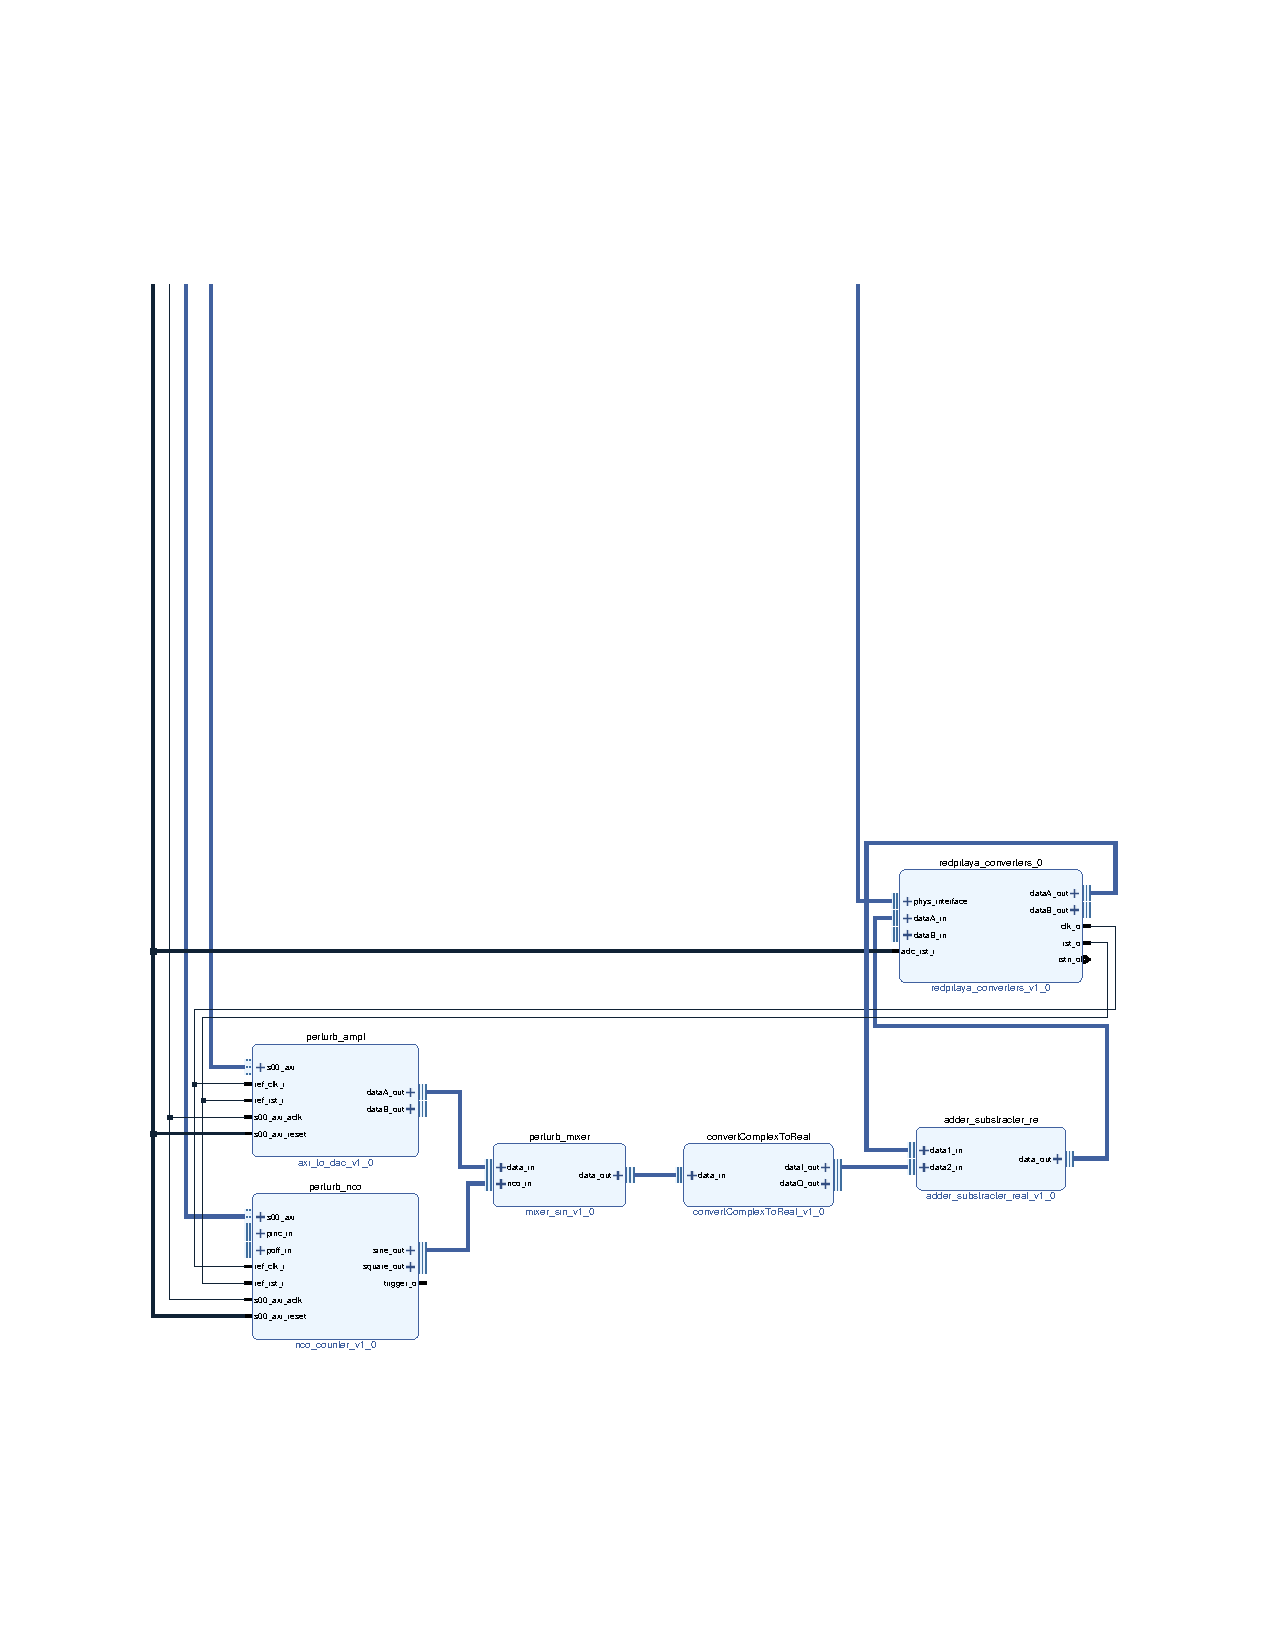
\includegraphics[width=16cm,trim={2.5cm 5cm 2.5cm 14cm}, clip]{design/mod_ampl.pdf}
		\caption{Part of the block diagram for the amplitude modulation.}
		\label{fig:mod_ampl}
	\end{center}
\end{figure}

\newpage
\subsection{IP configuration}
\vspace{0cm}
IPs configuration in this example:
\begin{center}
	\begin{tabular}{|>{\centering\arraybackslash}m{.3\linewidth} | >{\centering\arraybackslash}m{.3\linewidth} |}
		\hline
		IP & Configuration \\
		\hline
		& Counter size: $40~bits$\\ perturb\_nco &Data size: $16~bits$\\ &Lut size: $12~bits$ \\
		\hline
		perturb\_ampl&Data size: $14~bits$ \\
		\hline
		perturb\_mixer&Data in/out size: $14~bits$ \newline Nco\_size: $16~bits$ \\
		\hline
		& Data size: $14~bits$\\adder\_substracter\_re & Operation: add\\ &Format: Signed \\
		\hline
		convert$\mathbb{C}$to$\mathbb{R}$\_1&Data size: $14~bits$\\
		\hline
	\end{tabular}
\end{center}
\vspace{0cm}
\newpage
\subsection{Webserver configuration}


\begin{figure}[!h!tb]
	\begin{center}
		\includegraphics[width=14cm]{webserver/2020-01-13-104008_907x265_scrot.png}
		\caption{Screenshot of the sine perturbation part of the webserver.}
		\label{fig:amplModWs}
	\end{center}
\end{figure}
\vspace{-0.5cm}

\subsection{Expected output}
We use at the input a sine signal of $5~MHz$ and $0~dBm$.
With a sine perturbation of $50~MHz$ and $1000~arb.~unit$, we expect:

\begin{figure}[!h!tb]
	\begin{center}
		\includegraphics[width=14cm]{scope/Mod_amplOk.pdf}
		\caption{Expected behavior with input sine at $5~MHz$ and sine perturbation of $50~MHz$.}
		\label{fig:ampleModOK}
	\end{center}
\end{figure}
\vspace{-0.5cm}
\subsection{Unexpected output}

An unexpected situation can be the output signal visible in fig.\ref{fig:ampleModPasOK}: 

\begin{figure}[!h!tb]
	\begin{center}
		\includegraphics[width=14cm]{scope/Mod_amplPasOk.pdf}
		\caption{Unexpected behavior with input sine at $5~MHz$ and sine perturbation of $50~MHz$.}
		\label{fig:ampleModPasOK}
	\end{center}
\end{figure}

This situation is very similar to the fig.\ref{fig:doubleDDSpasOk} in subsection \ref{subsect:doubleDDSpasOk}: this output is a result of an overflow happening during the signal processing. This situation is due to an input signal too powerful with respect to the perturbation amplitude.
Solution: decrease the perturbation amplitude or the power of the input signal. 


\section{Frequency and phase modulation of a NCO}\label{sect:FMPM}

A frequency and a phase modulation can also be performed using the phase increment and the phase offset input of the NCO. The scheme presented below corresponds to the block diagram presented in fig.\ref{fig:mod_phase}.

\begin{figure}[h!tbp]
	\begin{center}
		\vspace{-3.5cm}
		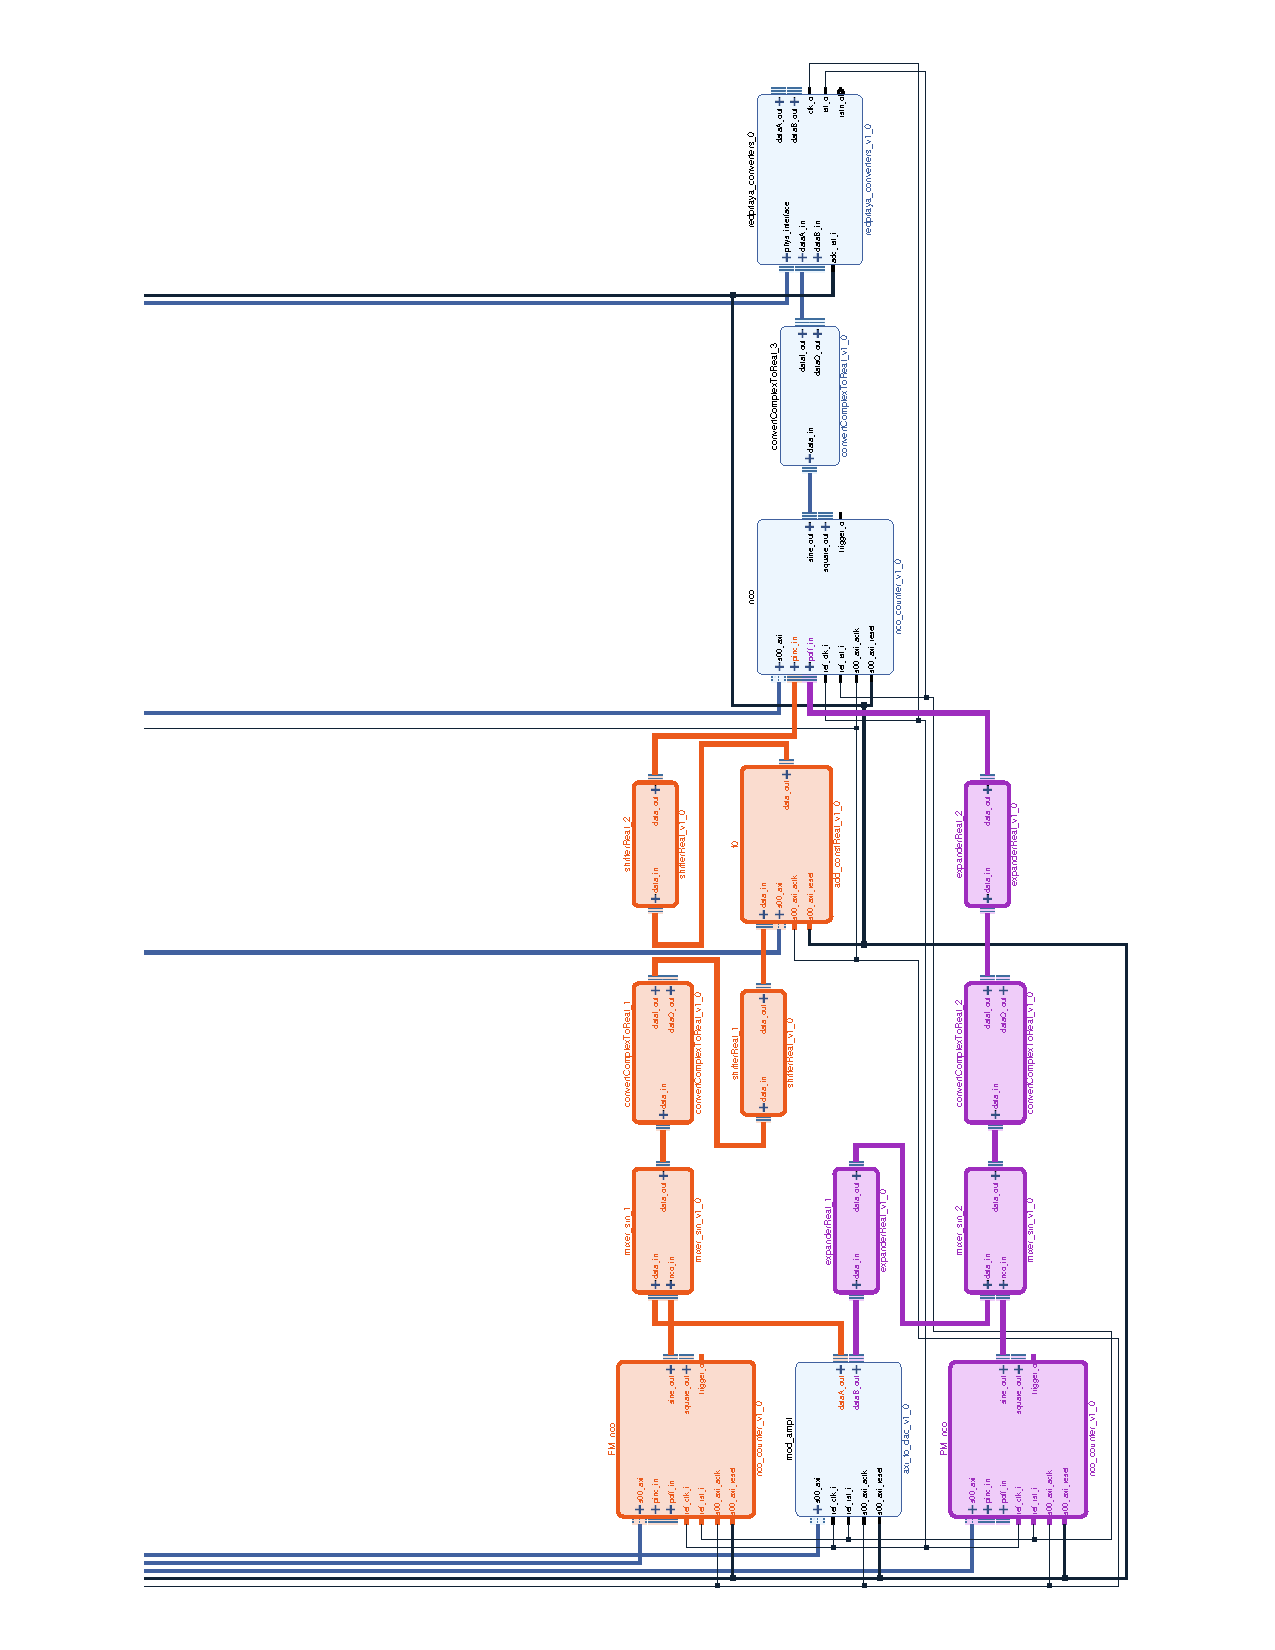
\includegraphics[width=8.4cm,trim={10cm 1cm 2.5cm 0cm}, clip]{design/FMPM3.pdf}
		\caption{Part of the block diagram for frequency (orange) and phase (purple) modulation of a NCO.}
		\label{fig:mod_phase}
	\end{center}
\end{figure}


\begin{center}
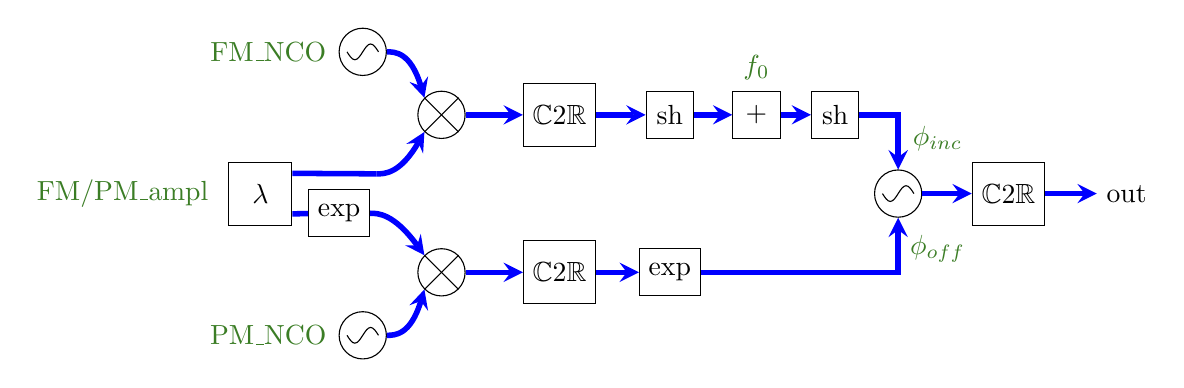
\begin{tikzpicture}	
\node [circle, draw ,minimum size=.6cm] (osc1){};
\draw ([xshift=-0.2cm] osc1.center) sin ([xshift=-0.10cm, yshift=-0.10cm] osc1.center) cos (osc1.center) sin ([xshift=0.10cm, yshift=0.10cm] osc1.center) cos ([xshift=0.2cm] osc1.center);

\node[draw, rectangle, minimum size=0.8cm, xshift=0.4cm, right of=osc1] (datout) {$\mathbb{C}$2$\mathbb{R}$};
\node[right of=datout, xshift=0.5cm] (o1) {out};
\draw [->,>=stealth,line width=2pt,blue] (osc1) -- (datout);
\draw [->,>=stealth,line width=2pt,blue] (datout) -- (o1);

\node[draw, rectangle, minimum size=.6cm, left of=osc1, xshift=0.2cm, above of=osc1] (plus) {sh};
\node[draw, rectangle, minimum size=.6cm, left of=plus] (plus1) {$+$};
\draw [->,>=stealth,line width=2pt,blue] (plus.east) -| (osc1.north);

\node[draw, rectangle, minimum size=0.8cm, xshift=-0.5cm, left of=plus1, left of=plus1] (dat) {$\mathbb{C}$2$\mathbb{R}$};
\node[draw, rectangle, minimum size=0.8cm, xshift=-4.3cm, below of=osc1] (dat1) {$\mathbb{C}$2$\mathbb{R}$};

\node[draw, rectangle, minimum size=.6cm, right of=dat, xshift=0.4cm] (sh1) {sh};
\node[draw, rectangle, minimum size=.6cm, right of=dat1, xshift=0.4cm] (exp2) {exp};

\node [circle, draw ,minimum size=.6cm, xshift=-0.5cm, left of=dat] (mix1) {};
\draw [-] (mix1.south west) -- (mix1.north east);
\draw [-] (mix1.south east) -- (mix1.north west);
\node [circle, draw ,minimum size=.6cm, xshift=-0.5cm, left of=dat1] (mix2) {};
\draw [-] (mix2.south west) -- (mix2.north east);
\draw [-] (mix2.south east) -- (mix2.north west);


\node[above of=plus1, yshift=-0.4cm] (f0) {{\color{OliveGreen}$f_0$}};

\draw [->,>=stealth,line width=2pt,blue] (mix1) -- (dat);
\draw [->,>=stealth,line width=2pt,blue] (dat) -- (sh1);
\draw [->,>=stealth,line width=2pt,blue] (sh1) -- (plus1);
\draw [->,>=stealth,line width=2pt,blue] (plus1) -- (plus);
\draw [->,>=stealth,line width=2pt,blue] (mix2) -- (dat1);
\draw [->,>=stealth,line width=2pt,blue] (dat1) -- (exp2);
\draw [->,>=stealth,line width=2pt,blue] (exp2) -| (osc1.south);

\node [circle, draw ,minimum size=.6cm, above of=mix1, left of=mix1, yshift=-0.2cm] (osc2){};
\draw ([xshift=-0.2cm] osc2.center) sin ([xshift=-0.10cm, yshift=-0.10cm] osc2.center) cos (osc2.center) sin ([xshift=0.10cm, yshift=0.10cm] osc2.center) cos ([xshift=0.2cm] osc2.center);

\node [circle, draw ,minimum size=.6cm, below of=mix2, left of=mix2, yshift=0.2cm] (osc3){};
\draw ([xshift=-0.2cm] osc3.center) sin ([xshift=-0.10cm, yshift=-0.10cm] osc3.center) cos (osc3.center) sin ([xshift=0.10cm, yshift=0.10cm] osc3.center) cos ([xshift=0.2cm] osc3.center);

\node[draw, rectangle, minimum size=0.8cm, left of=osc1, xshift=-7.1cm] (mampl) {$\lambda$};
\node[draw, rectangle, minimum size=.6cm, right of=mampl, yshift=-0.25cm] (exp1) {exp};
\node[right of=mampl, xshift=0.6cm, yshift=0.25cm] (exp3) {};
\draw [-,line width=2pt,blue] ([yshift=0.15cm] mampl.south east) -- (exp1);
\draw [-,line width=2pt,blue] ([yshift=-0.15cm] mampl.north east) -- (exp3);

\draw [->, >=stealth, line width=2pt, blue] (osc2.east) .. controls ([xshift=0.1cm, yshift=0cm] osc2.east) and ([xshift=0.3cm, yshift=0cm] osc2.east) ..(mix1.north west);
\draw [->, >=stealth, line width=2pt, blue] (osc3.east) .. controls ([xshift=0.1cm, yshift=0cm] osc3.east) and ([xshift=0.3cm, yshift=0cm] osc3.east) ..(mix2.south west);

\draw [->, >=stealth, line width=2pt, blue] (exp1.east) .. controls ([xshift=0.1cm, yshift=0cm] exp1.east) and ([xshift=0.3cm, yshift=0cm] exp1.east) ..(mix2.north west);

\draw [->, >=stealth, line width=2pt, blue] (exp3.west) .. controls ([xshift=0.1cm, yshift=0cm] exp3.west) and ([xshift=0.3cm, yshift=0cm] exp3.west) ..(mix1.south west);

\node[left of=osc2, xshift=-0.2cm] () {{\color{OliveGreen}FM\_NCO}};
\node[left of=osc3, xshift=-0.2cm] () {{\color{OliveGreen}PM\_NCO}};
\node[left of=mampl, xshift=-0.75cm] () {{\color{OliveGreen}FM/PM\_ampl}};
\node[xshift=+0.5cm, yshift=+0.7cm] () {{\color{OliveGreen}$\phi_{inc}$}};
\node[xshift=+0.5cm, yshift=-0.7cm] () {{\color{OliveGreen}$\phi_{off}$}};
\end{tikzpicture} \\
\end{center}


\vspace{-0.2cm}
\subsection{IP configuration}
%\vspace{0.5cm}
IPs configuration in this example:


\begin{center}
	\begin{tabular}{|>{\centering\arraybackslash}m{.3\linewidth} | >{\centering\arraybackslash}m{.3\linewidth} |}
		\hline
		IP & Configuration \\
		\hline
		& Counter size: $40~bits$\\ FP\_nco/PM\_nco/nco &Data size: $16~bits$\\ &Lut size: $12~bits$ \\
		\hline
		mod\_ampl&Data size: $27~bits$ \\
		\hline
		& Data in size: $27~bits$\\expanderReal\_1 & Data in size: $16~bits$\\ &Format: Signed \\
		\hdashline
		& Data in size: $16~bits$\\expanderReal\_2 & Data in size: $12~bits$\\ &Format: Signed \\
		\hline
		shiftReal\_1&Data in size: $27~bits$ \newline data out size: $32~bits$ \\
		\hdashline
		shiftReal\_2&Data in size: $32~bits$ \newline data out size: $40~bits$ \\
		\hline
		mixer\_sin\_1&Data in/out size: $27~bits$ \newline Nco\_size: $16~bits$ \\
		\hdashline
		mixer\_sin\_2&Data in/out size: $16~bits$ \newline Nco\_size: $16~bits$ \\
		\hline
		$f_0$&Data in/out size: $32~bits$ \newline Format: Signed \\
		\hline
		convert$\mathbb{C}$to$\mathbb{R}$\_1&Data size: $27~bits$\\
		\hdashline
		convert$\mathbb{C}$to$\mathbb{R}$\_2&Data size: $16~bits$\\
		\hdashline
		convert$\mathbb{C}$to$\mathbb{R}$\_3&Data size: $14~bits$\\
		\hline
	\end{tabular}
\end{center}

\vspace{0.5cm}
\subsection{Webserver configuration}

Here, only the PM\_deviation is reconfigured between $-8192$ and $8191~arb.~unit$. Both FM\_nco, PM\_nco, f0, FM\_deviation and nco are configured between $0$ and $62000000~Hz$. The webserver is represented in fig.\ref{fig:FMPMwebserver}

\begin{figure}[h!tb]
	\begin{center}
		\vspace{0.5cm}
		\includegraphics[width=14cm,trim={0cm 0cm 0cm 0cm}, clip]{webserver/2020-01-07-090526_907x561_scrot.png}
		\caption{Screenshot of the phase and frequency modulation webserver. "pinc" checkbox is unchecked: frequency modulation.}
		\label{fig:FMPMwebserver}
	\end{center}
\end{figure}

\subsection{Expected frequency modulation}

For the frequency modulation, we use the phase increment input of the nco. In the webserver this requires to uncheck the "pinc" checkbox. This means that the phase increment is external and whatever is the frequency mentioned in /dev/nco, it will not be taken into consideration. In this case, the frequency of the carrier must be written in /dev/f0: this adds to the FM\_nco a constant corresponding to the carrier frequency. 
\newline\newline
To show an exaggerated example of the frequency modulation, we use a carrier frequency f0 of $5~MHz$. The frequency of the FM\_nco and the FM\_deviation must remain lower than the carrier frequency. Here we used a frequency modulation of $200~kHz$ and a deviation of $4~MHz$. We expect the following output: 

\begin{figure}[!h!tb]
	\begin{center}
		\includegraphics[width=14cm]{scope/Mod_freqOk.pdf}
		\caption{Expected frequency modulation with a carrier at $5~MHz$, and a deviation of $4~MHz$.}
		\label{fig:FMModOK}
	\end{center}
\end{figure}

\subsection{Expected phase modulation}

For the phase modulation, we use the phase offset input of the nco and keep an internal phase increment. In the webserver this requires to uncheck the "poff" checkbox and keep checked the "pinc" checkbox. This means this time that the phase offset is external, and the nco frequency taken into consideration is the one mentionned in /dev/nco. The phase offset range goes from $-4\pi$ to $4\pi$, therefore a PM\_deviation of $\pm 8191~arb.~unit$ corresponds approximately to deviation of $\pm 4 \pi$. 
\newline\newline
The example in fig.\ref{fig:PMModOK} represents a phase modulation for a carrier at $1~MHz$, a deviation slightly below $2\pi$ (PM\_deviation = $4000~arb.~unit$), and a modulation frequency of $100~kHz$.

\begin{figure}[!h!tb]
	\begin{center}
		\includegraphics[width=14cm]{scope/Mod_phaseOk.pdf}
		\caption{Expected phase modulation with a carrier at $1~MHz$, and a deviation of $2 \pi$..}
		\label{fig:PMModOK}
	\end{center}
\end{figure}

\subsection{Unexpected output}

Unexpected outputs or a lack of signal can have several origins. Here is a non-exhaustive list of unexpected situations, and the potential solutions:

\begin{itemize}
	\setlength\itemsep{-0.0cm}
	\item The observed deviation is higher or lower than expected: \newline \hspace*{1cm}  \textit{The data sizes in the expanders/shifters in the block design are chosen so that the range of the mod\_ampl block fit with the phase increment/offset inputs of the nco. If the deviation is not the one expected, check if the data sizes between the mod\_ampl block and the nco block are adapted.}
	\item There is no output signal or the signal is fixed: 
\textit{\vspace{-0.25cm}	\begin{enumerate}
		\setlength\itemsep{-0.0cm}
		\item Check the connections in the block design.
		\item Check if the data sizes are adapted.
		\item Check if the mod\_ampl block (axi\_to\_dac block) is configured to have a data output always enabled: its state must remain high.
	\end{enumerate}}
	\item There seems to be an amplitude modulation with the frequency/phase modulation, or the output amplitude seems to vary with the frequency. \newline \hspace*{1cm}  \textit{The input impedance of your monitoring device may be quite low.}
\end{itemize}

\section{Filtering}\label{sect:filtering}

The FIR (Finite Impulse Response) filter has the role of filter with a number of coefficients that is configurable during the creation of a design. Similarly to the mean block that makes a moving average, the FIR has a decimation option. The decimation is performed before the filtering and slows the data flow. To learn more about the FIR, visit: https://github.com/oscimp/oscimpDigital/tree/master/doc/tutorials/redpitaya/4-FIR

\subsection{Calculation of the coefficients}

The number of coefficients and their values determine the transfer function of the FIR. Therefore the coefficient must be calculated according to the situation. Also, the coefficients must be integers with a size determined in the FIR block, by default and in our case on $16~bits$ including one bit dedicated to the sign. 
\newline\newline
To compute the FIR coefficients, octave proposes the signal package\footnote{https://octave.sourceforge.io/signal/index.html} with the function fir1\footnote{https://octave.sourceforge.io/signal/function/fir1.html} that allows to design either lowpass, highpass, bandpass or bandstop filters. First, load the signal package of octave:

\vspace{-0.1cm}
\begin{lstlisting}
octave:1> pkg load signal
\end{lstlisting}
\vspace{+0.5cm}

Then the syntax is as follows:

\vspace{-0.1cm}
\begin{lstlisting}
COEFF = fir1(n, w, type)
\end{lstlisting}
\vspace{+0.5cm}

With $n$ the order of the filter, resulting in $n+1$ coefficients, $w$ the normalized cutoff frequency(ies), and $type$ the type of the filter "low", "high", "stop" or "pass". 

For example, the calculation of $10$ coefficients ($9th$ order filter) on $16~bits$ ($\times 2^{15}$, without the bit dedicated to the sign) for a lowpass filter with a cutoff frequency at the half range ($0.5$), gives the following output: 

\vspace{-0.1cm}
\begin{lstlisting}
octave:2> COEFF = transpose(int16(fir1(9,0.5)*2**15))
COEFF =
128
-397
-1337
3775
14214
14214
3775
-1337
-397
128
\end{lstlisting}
\vspace{+0.5cm}

It should be noted that the FIR coefficients are recognizable by their symmetry. The function freqz of the signal package allows to obtain and visualize the frequency and phase responses of the designed FIR coefficients. Some examples are represented below:
\newline\newline
\underline{Lowpass filter with $55$ coefficients}\newline\newline
Filter of $54th$ order. The cutoff frequency of $3~MHz$ is calculated on the basis of a sampling frequency of $125~MHz$, i.e. a Nyquist frequency of $62.5~MHz$. Then the cutoff is $3/62.5=0.048$. In the following, freqz has $4$ arguments. The first is our FIR coefficients. The second represents the coefficients of feedback of an IIR (Infinite Impulse Response) filter, here the value $1$ means we consider a simple FIR. The third ($1024$) is the resolution of the frequency/phase response diagram, and the last is the sampling frequency $125~MHz$:

\vspace{-0.1cm}
\begin{lstlisting}
octave:2> figure(1); freqz(int16(fir1(54,0.048)*2**15),1,1024,125e6)
\end{lstlisting}
\vspace{-0cm}

\begin{figure}[!h!tb]
	\begin{center}
		\includegraphics[width=10.5cm,trim={1.5cm 6.9cm 1.5cm 7cm}, clip]{curves/lp55co.pdf}
		\caption{Lowpass filter at a $3~MHz$ cutoff frequency with $55$ coefficients.}
		\label{curv:LP}
	\end{center}
\end{figure}

The importance of designing the filter coefficients adapted to one precise situation is clearly visible here, since the blocking range is not flat but constituted of small bounces. The rejection between the top and the bottom of the bounces can exceed $20~dB$ depending on the FIR coefficients. Thus, it is interesting to design the FIR coefficients so that it rejects a precise spectral component (such as harmonics).
\newline\newline
\underline{Lowpass filter with $15$ coefficients}\newline\newline
The effect of the number of coefficient can be seen by designing the same fir with much less coefficients, here $15$ coefficients:

\vspace{-0.1cm}
\begin{lstlisting}
octave:3> figure(2); freqz(int16(fir1(14,0.048)*2**15),1,1024,125e6)
\end{lstlisting}
\vspace{-0cm}

\begin{figure}[!h!tb]
	\begin{center}
		\includegraphics[width=12cm,trim={1.5cm 6.9cm 1.5cm 7cm}, clip]{curves/lp15co.pdf}
		\caption{Lowpass filter at a $3~MHz$ cutoff frequency with $15$ coefficients.}
		\label{curv:LP2}
	\end{center}
\end{figure}
\vspace{-0.5cm}
In this case, the whole rejection of the filter is lower, and the filtering less precise.
\newline\newline
\underline{Dual bandstop filter}\newline\newline
Example of syntax for the designing of a more exotic filter. Here a filter with two stop bands at $5~MHz-25~MHz$ and $40~MHz-50~MHz$:

\vspace{-0.1cm}
\begin{lstlisting}
octave:4> figure(3); freqz(int16(fir1(54,[0.08 0.4 0.64 0.8],'stop')*2**15),1,1024,125e6)
\end{lstlisting}
\vspace{-0cm}

\begin{figure}[!h!tb]
	\begin{center}
		\includegraphics[width=12cm,trim={1.5cm 6.9cm 1.5cm 7cm}, clip]{curves/bs55co.pdf}
		\caption{Bandstop filter at at $5~MHz-25~MHz$ and $40~MHz-50~MHz$, with $55$ coefficients.}
		\label{curv:DSP}
	\end{center}
\end{figure}

\subsection{Loading of the coefficients}
\vspace{0.5cm}
The loading of the coefficients in the FIR is performed in our case using the function visible in the /oscimpDigital/lib/fir\_conf.h file :

\vspace{-0cm}
\begin{lstlisting}[language=C]
fir_send_confSigned(const char *basename, const char *fileCoeff, const int coeffSize);
\end{lstlisting}
\vspace{0.6cm} 

In the python wrapper liboscimp\_fpga.py (see section \ref{sect:webserver}), it takes the form:

\vspace{-0cm}
\begin{lstlisting}[language=Python]
def fir_send_confSigned(basename, nbFir,fileCoeff, coeffSize):
		file = ctypes.create_string_buffer(str.encode(basename))
		coeffFile = ctypes.create_string_buffer(str.encode(fileCoeff))
		lib.fir_send_confSigned(file, nbFir, coeffFile, coeffSize)
\end{lstlisting}
\vspace{0.6cm}

Where coeffFile is a data file where the FIR coefficients are stored in column, and coeffSize the number of coefficients mentioned in the FIR block and contained in coeffFile.
Then an example of python script to load one FIR with $N$ coefficients stored in the My\_FIR\_coefficients.dat file is :
\vspace{+0.8cm}
\begin{lstlisting}[language=Python]
#!/usr/bin/env python

import liboscimp_fpga

liboscimp_fpga.fir_send_confSigned('/dev/MY_FIR_FILE', 'My_FIR_coefficients.dat', N)
\end{lstlisting}
\vspace{0.5cm}

\section{Demodulation}\label{sect:demod}

A demodulation in amplitude or frequency/phase can be performed using the scheme below: 

\begin{center}
	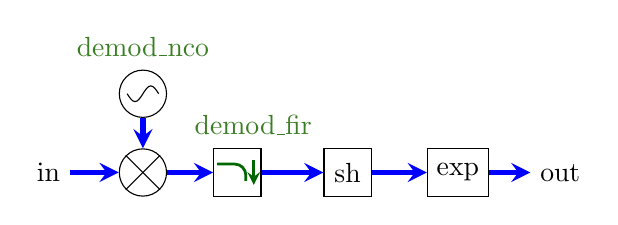
\begin{tikzpicture}	
	\node [circle, draw ,minimum size=.6cm] (osc1){};
	\node [above of=osc1, yshift=-0.4cm] {{\color{OliveGreen}demod\_nco}};
	\draw ([xshift=-0.2cm] osc1.center) sin ([xshift=-0.10cm, yshift=-0.10cm] osc1.center) cos (osc1.center) sin ([xshift=0.10cm, yshift=0.10cm] osc1.center) cos ([xshift=0.2cm] osc1.center);

	\node [circle, draw ,minimum size=.6cm, below of=osc1] (mix2) {};
	\draw [-] (mix2.south west) -- (mix2.north east);
	\draw [-] (mix2.south east) -- (mix2.north west);
	
	\node[xshift=0.8cm, left of=mix2, xshift=-1cm] (i1) {in};
	\draw [->,>=stealth,line width=2pt,blue] (i1) -- (mix2);
	\draw [->,>=stealth,line width=2pt,blue] (osc1) -- (mix2);
	
	\node[draw, rectangle, minimum size=.6cm, right of=mix2, xshift=0.2cm] (fir) {};
	\draw [-, line width=1pt, color=black!60!green, rounded corners] ([xshift=.05cm,yshift=-.2cm] fir.north west) -| ([xshift=-.2cm,yshift=+.2cm] fir.south east);
	\draw [->,>=stealth, line width=1pt, color=black!60!green] ([xshift=-.1cm,yshift=-.15cm] fir.north east) -- ([xshift=-.1cm,yshift=+.15cm] fir.south east);
	\draw [->,>=stealth,line width=2pt,blue] (mix2) -- (fir);
	\node [above of=fir, yshift=-0.4cm, xshift=0.2cm] {{\color{OliveGreen}demod\_fir}};
	
	\node[draw, rectangle, minimum size=.6cm, right of=fir, xshift=0.4cm] (sh) {sh};
	\node[draw, rectangle, minimum size=.6cm, right of=sh, xshift=0.4cm] (exp) {exp};
	
	\node[xshift=0.8cm, right of=exp, xshift=-0.5cm] (o1) {out};
	\draw [->,>=stealth,line width=2pt,blue] (fir) -- (sh);
	\draw [->,>=stealth,line width=2pt,blue] (sh) -- (exp);
	\draw [->,>=stealth,line width=2pt,blue] (exp) -- (o1);
	\end{tikzpicture} 
\end{center}

The FIR is configured as a lowpass filter, to reject mainly the sum frequency component after mixing.
The block diagram corresponding to this scheme is presented in fig.\ref{fig:demod}.

\begin{figure}[h!tb]
	\begin{center}
		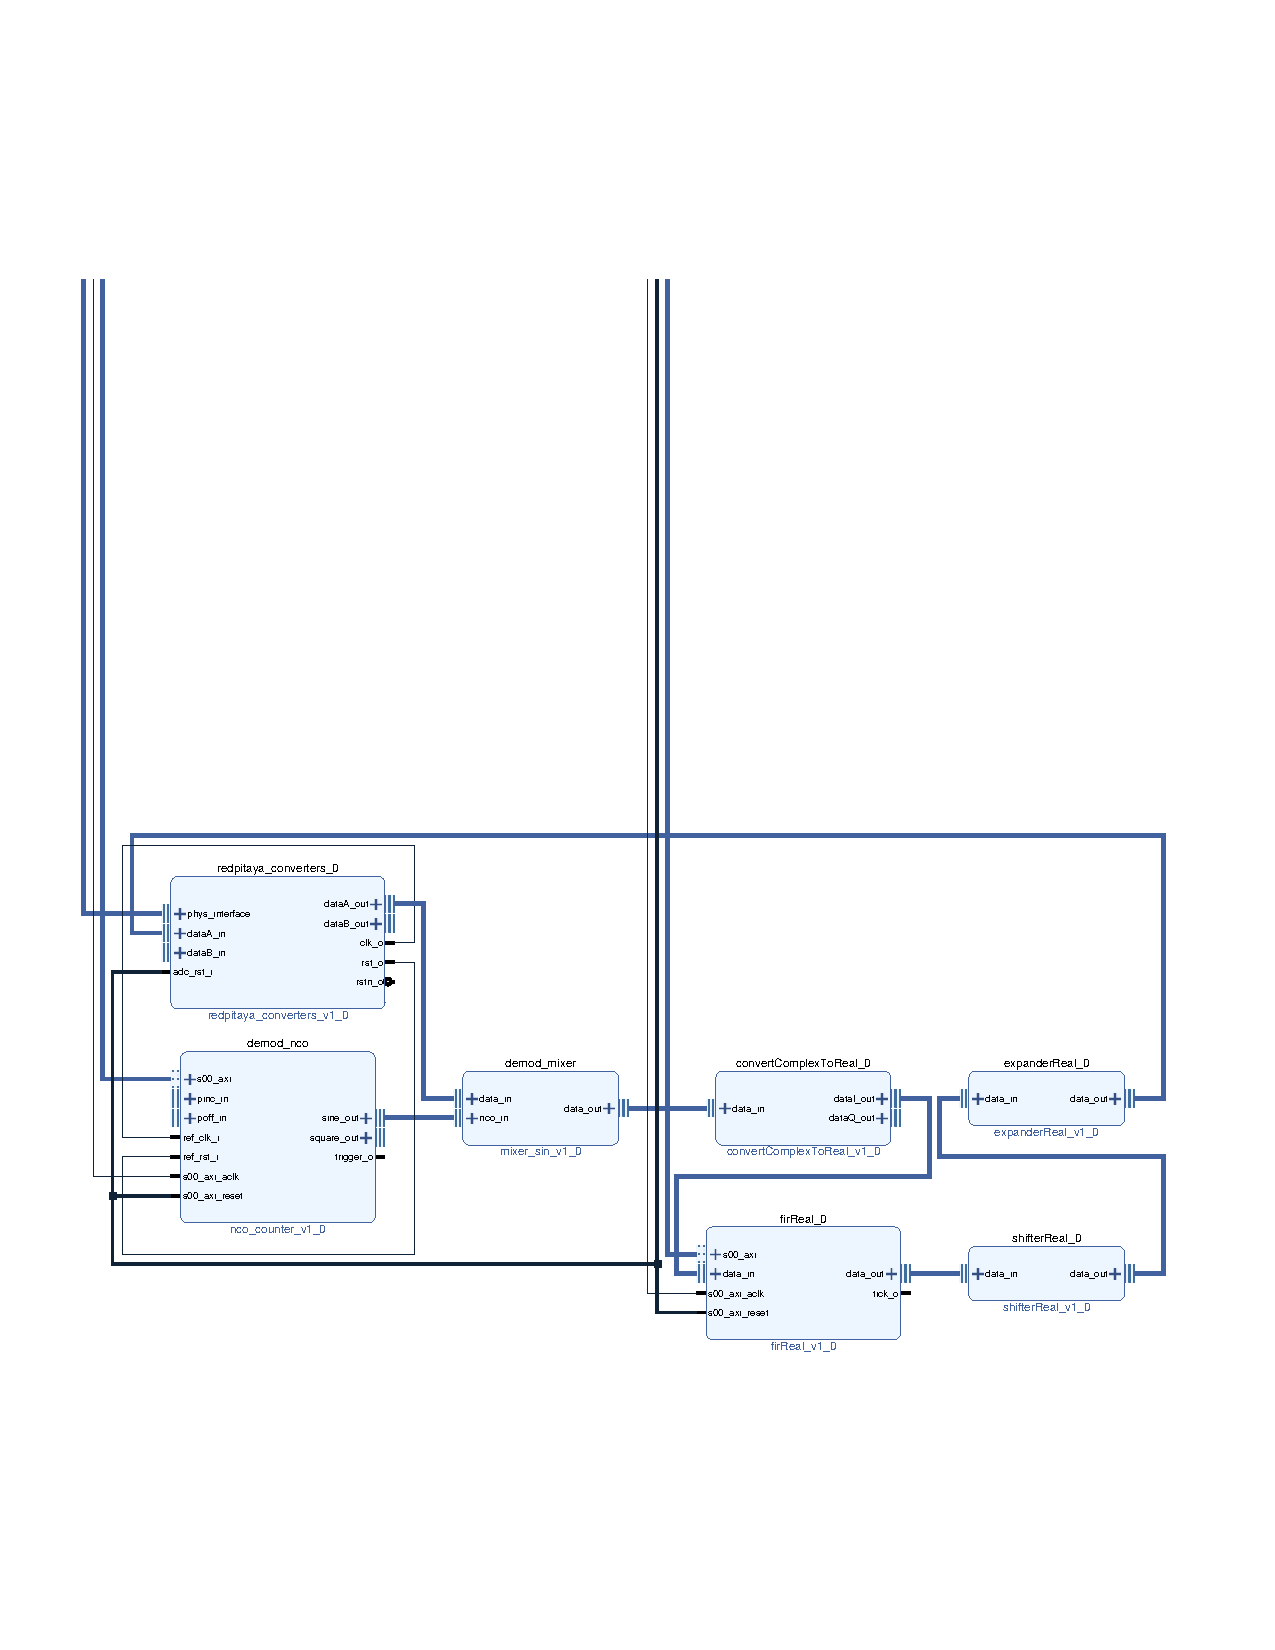
\includegraphics[width=15cm,trim={1.3cm 5cm 1.5cm 13.8cm}, clip]{design/demod.pdf}
		\caption{Part of the block diagram for the demodulation, including the filtering.}
		\label{fig:demod}
	\end{center}
\end{figure}

\vspace{-0.3cm}
\subsection{IP configuration}

The IPs configuration in this example is given in the following table :

\begin{center}
	\begin{tabular}{|>{\centering\arraybackslash}m{.3\linewidth} | >{\centering\arraybackslash}m{.3\linewidth} |}
		\hline
		IP & Configuration \\
		\hline
		& Counter size: $40~bits$\\ demod\_nco &Data size: $16~bits$\\ &Lut size: $12~bits$ \\
		\hline
		demod\_mixer&Data in/out size: $14~bits$ \newline Nco\_size: $16~bits$ \\

		\hline
		convert$\mathbb{C}$to$\mathbb{R}$\_1&Data size: $14~bits$\\
		\hline
		&COEFF Size: $16~bits$\\&Data In size: $14~bits$\\demod\_fir& Data Out size: $32~bits$\\&Decim Factor: $1$\\&Nb COEFF: $55$\\
		\hline
		shiftReal\_0&Data in size: $32~bits$ \newline Data out size: $18~bits$\\
		\hline
		expanderReal\_0&Data in size: $18~bits$ \newline Data out size: $14~bits$\\
		\hline
	\end{tabular}
\end{center}
\vspace{0.2cm}
The FIR coefficients used in this section are the one calculated for the $55$ coefficients lowpass filter given at the previous section. Then the data sizes assigned to the shifter and expander blocks, are chosen to maximize the range of the output signal for a maximum input amplitude. Those parameters must also be adapted depending on the FIR coefficients to avoid an overflow. In the case the block design must remain adapted to several situations, a dynamic shifter can be used instead of the succession shifter + expander. It allows choosing from the webserver the beginning of the $14~bits$ output word among the $32$ output bits of the FIR, and therefore choosing the output range. 

\vspace{0.2cm}

\subsection{Webserver configuration}
\vspace{-0.3cm}
\begin{figure}[h!tb]
	\begin{center}
		\vspace{0.5cm}
		\includegraphics[width=15cm,trim={0cm 0cm 0cm 0cm}, clip]{webserver/2020-01-08-082405_907x201_scrot.png}
		\caption{Screenshot of the demodulation webserver: only one nco is controlled here.}
		\label{fig:demod_webserver}
	\end{center}
\end{figure}
\vspace{-1cm}

\subsection{Expected output}

To make small review of the behavior of this demodulation setup, we display here four cases:

\begin{itemize}
	\setlength\itemsep{-0.2cm}
	\item Mix of two sine signal (i.e. not a demodulation)
	\item Demodulation of an unmodulated sine signal
	\item Amplitude demodulation
	\item Frequency demodulation
\end{itemize}

\underline{Mix of two sine signal}\newline

A first test that can be done with this setup, is the mixing of two sine signal. The beatnote of the two signals shows the range of the output signal. If the output signal is too weak or if there is an overflow, then the data sizes of the expander and shifter blocks must be changed.\newline


\underline{Demodulation of an unmodulated sine signal}\newline

The type of demodulation depends on the phase shift between the two signals. To show the effect of this phase shift on the demodulated signal, we show here the demodulation of an unmodulated sine signal. In this example the input is a simple sine signal at $40~MHz$, thus the demodulation frequency is set to $40~MHz$. The phase offset of the demodulation signal allows changing the phase shift between the two signals. Then the output signal is a direct signal whose amplitude depend on the phase shift between the two signals.
\newline\newline
First, with a demodulation phase offset of $1550$, the signals are \textbf{in phase}. Then the amplitude of the output signal is maximum:

\begin{figure}[!h!tb]
	\begin{center}
		\includegraphics[width=13cm,trim={0cm 0cm 0cm 0cm}, clip]{scope/demods1.pdf}
		\caption{The carrier and the demodulation signal are in phase.}
		\label{curv:demodsine1}
	\end{center}
\end{figure}

Secondly, with a demodulation phase offset of $3600$, the signals are \textbf{in antiphase}. Then the amplitude of the output signal is minimum:
\newline

\begin{figure}[!h!tb]
	\begin{center}
		\includegraphics[width=13cm,trim={0cm 0cm 0cm 0cm}, clip]{scope/demods2.pdf}
		\caption{The carrier and the demodulation signal are in antiphase.}
		\label{curv:demodsine2}
	\end{center}
\end{figure}

Finally, with a demodulation phase offset of $2500$, the signals are \textbf{in quadrature}. Then the amplitude of the output signal is zero:

\begin{figure}[!h!tb]
	\begin{center}
		\includegraphics[width=13cm,trim={0cm 0cm 0cm 0cm}, clip]{scope/demods3.pdf}
		\caption{The carrier and the demodulation signal are in quadrature.}
		\label{curv:demodsine3}
	\end{center}
\end{figure}


As a reminder, the phase offset allows a phase shift of $\pm 4\pi$, i.e. approximately $2048~arb.~unit$ between the "in phase" and "in antiphase" situations. The phase offsets mentioned above allows verifying that. However those phase offsets does not always correspond to the situations described, since the nco has an arbitrary phase. Therefore, it may be adjusted each time the nco status is modified. This point also applies to the input oscillator. 
\newline\newline
\underline{Amplitude demodulation}\newline\newline

For the amplitude demodulation, the carrier and the demodulation signal must be in phase. Here we use a carrier at $10~MHz$, and the modulating signal is a sine function at $50~kHz$, and a modulation depth of $50\%$:

\begin{figure}[!h!tb]
	\begin{center}
		\includegraphics[width=13cm,trim={0cm 0cm 0cm 0cm}, clip]{scope/demodampl.pdf}
		\caption{Amplitude demodulation.}
		\label{curv:demodampl}
	\end{center}
\end{figure}
\vspace{-0.8cm}
As it is visible on the fig.\ref{curv:demodampl}, a slight delay is visible between the input and the demodulated signal. This is due to the signal processing in the FPGA. 
\vspace{-0.1cm}
\newline\newline
\vspace{-0.1cm}
\underline{Phase demodulation}\newline\newline
For the phase demodulation, the carrier and the demodulation signal must be in quadrature In this example the carrier frequency is $10~MHz$, and the modulating signal is a square signal at $50~kHz$ with a deviation of $50^\circ$:

\begin{figure}[!h!tb]
	\begin{center}
		\includegraphics[width=13cm,trim={0cm 0cm 0cm 0cm}, clip]{scope/demodphcar.pdf}
		\caption{Phase demodulation.}
		\label{curv:demodph}
	\end{center}
\end{figure}

In this figure, only the transition between the two levels of the square is visible, at the time $-410~ns$ for the input signal and around $0~s$ for the output signal. This shows the delay due to the signal processing in the FPGA. In this example the delay is mostly due to the FIR, since it requires $55$ cycles to work, i.e. the number of coefficients of the FIR.

\subsection{Unexpected output}

\section{Monitoring}\label{sect:Monitoring}

In this section we show an example of use of the dataReal\_to\_ram block, used to monitor data. Basically monitoring a data flow only requires the dataReal\_to\_ram block, however we show a setup where the meanReal block is placed upstream to decimate/slow down the flow. The scheme is presented below:
 
\begin{center}
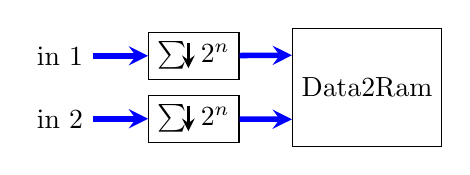
\begin{tikzpicture}
\node[draw, rectangle, minimum size=1.5cm] (dat) {Data2Ram};
\node[draw, rectangle, minimum size=.6cm, left of=dat, xshift=-1.2cm, yshift=+.4cm] (plus1) {$\sum~2^n$};
\draw [->,>=stealth, line width=1pt] ([xshift=-.65cm,yshift=-.15cm] plus1.north east) -- ([xshift=-.65cm,yshift=+.15cm] plus1.south east);
\node[draw, rectangle, minimum size=.6cm, left of=dat, xshift=-1.2cm,  yshift=-.4cm] (plus2) {$\sum~2^n$};
\draw [->,>=stealth, line width=1pt] ([xshift=-.65cm,yshift=-.15cm] plus2.north east) -- ([xshift=-.65cm,yshift=+.15cm] plus2.south east);
\node[left of=plus1, xshift=-0.7cm] (i1) {in 1};
\node[left of=plus2, xshift=-0.7cm] (i2) {in 2};
\draw [->,>=stealth,line width=2pt,blue] (plus1) -- ([yshift=-.35cm] dat.north west);
\draw [->,>=stealth,line width=2pt,blue] (plus2) -- ([yshift=+.35cm]dat.south west);
\draw [->,>=stealth,line width=2pt,blue] (i1) -- (plus1);
\draw [->,>=stealth,line width=2pt,blue] (i2) -- (plus2);
\end{tikzpicture} 
\end{center}

The block diagram corresponding to this scheme is as follows:

\begin{figure}[h!tb]
	\begin{center}
		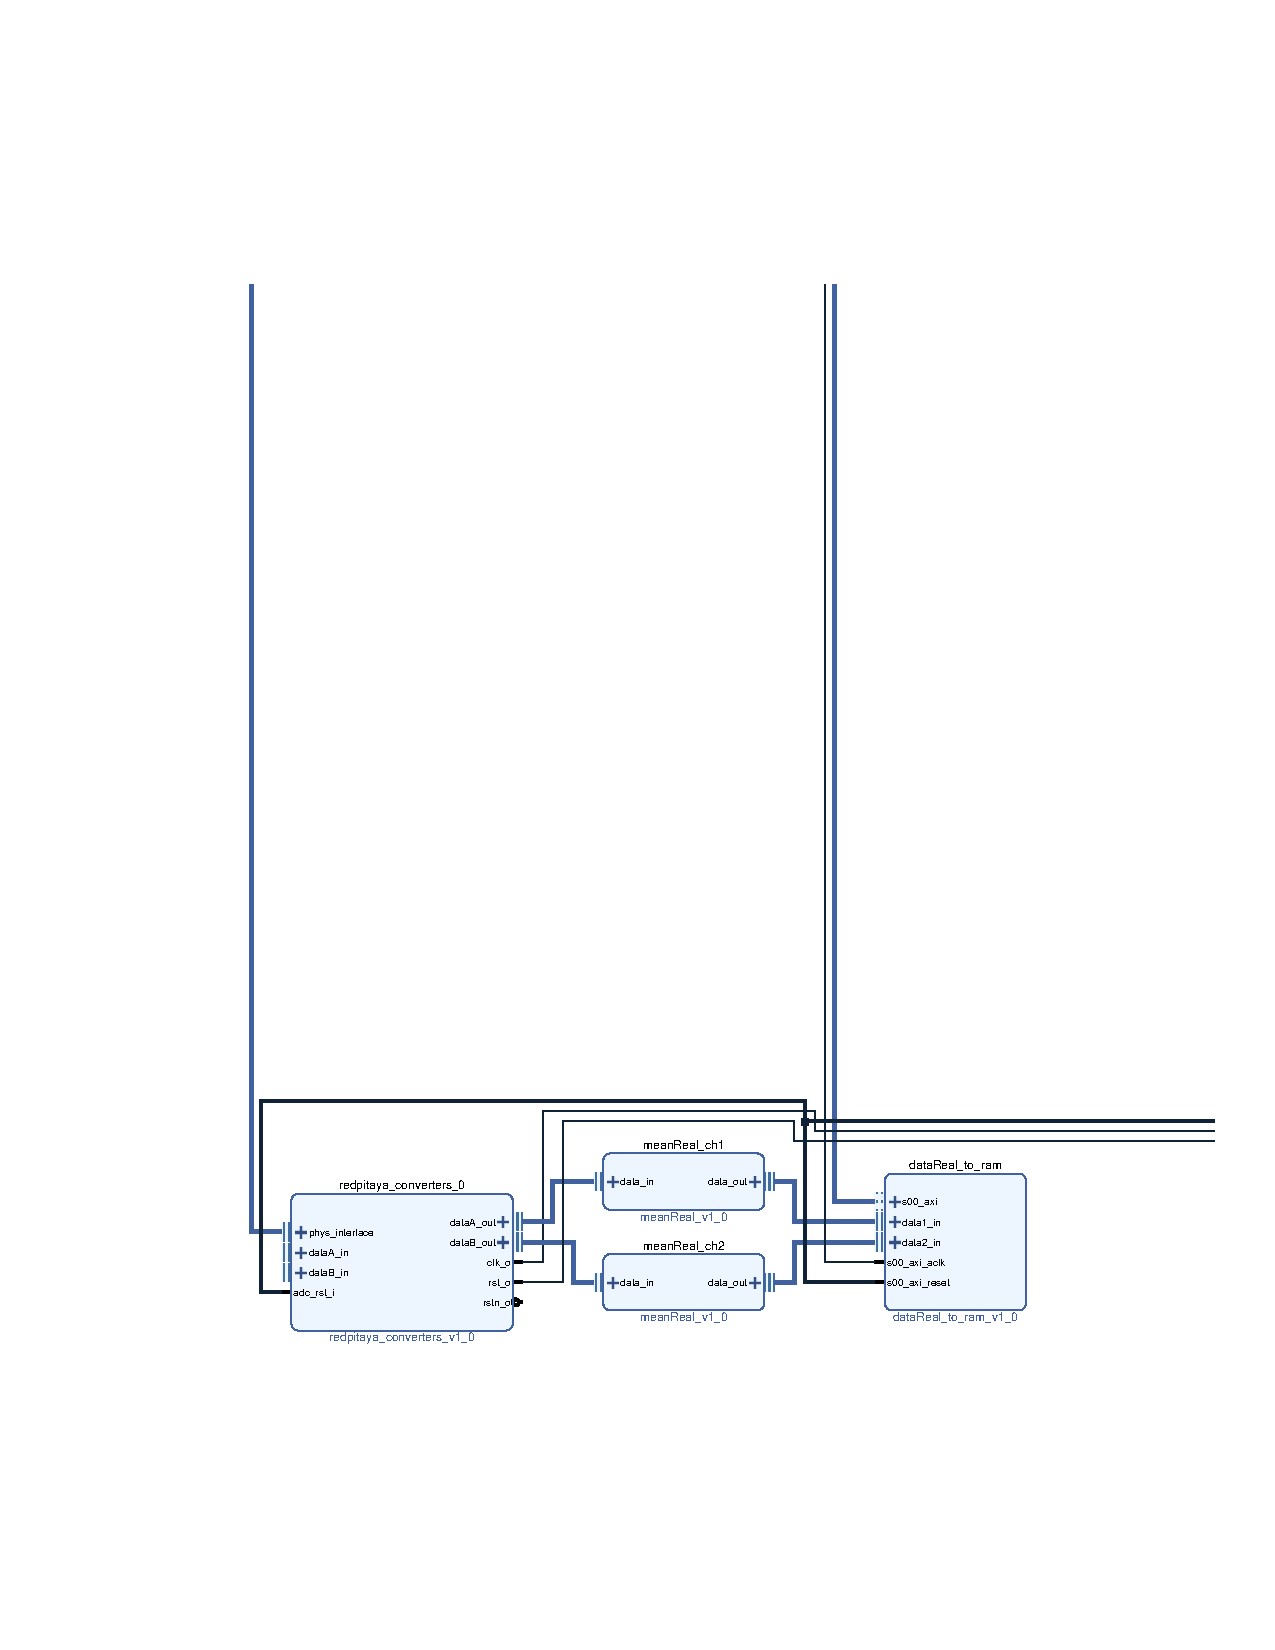
\includegraphics[width=15cm,trim={4cm 5cm 4cm 18cm}, clip]{design/data2ramMoy.pdf}
		\caption{Part of the block diagram for monitoring with the data2ram block.}
		\label{fig:data2ram}
	\end{center}
\end{figure}

For an average/decimation $\geq ~2$, this configuration results in spectral aliasing and is a disadvantage when used without filtering. However when the useful signal spreads on a shorter range than the spectral range available, it allows monitoring the data with more points than with a full range. 

\vspace{0.0cm}
\subsection{IP configuration}
he IPs configuration in this example is given in the following table :

\begin{center}
	\begin{tabular}{|>{\centering\arraybackslash}m{.3\linewidth} | >{\centering\arraybackslash}m{.3\linewidth} |}
		\hline
		dataReal\_to\_ram&Data size: $16~bits$ \newline Data format: signed\newline NB input: $2$\newline Nb Sample: $=~K$\\
		\hline
		meanReal\_ch1/2&Input Data size: $14~bits$ \newline Output Data Size: $16~bits$\newline Nb Accum: $=~2^n~bits$\newline Shift: $=~n~bits$\\
		\hline
	\end{tabular}
\end{center}
\vspace{0.2cm}

The number of samples of the dataReal\_to\_ram block, and the shift and number of accumulation of the meanReal blocks can vary upon the situations. Some examples will be listed in the expected output section (\ref*{sect:expOMon}). 

\subsection{Data reading}

The data stored in the data\_to\_ram buffer are C signed shorts, over $2~bytes$. With a data\_to\_ram configured with $2$ inputs and $K$ samples, this means the buffer contains ${4\times K~bytes}$. An example of reading of the data\_to\_ram block with a C script is presented here:
\newline
https://github.com/oscimp/oscimpDigital/tree/master/doc/tutorials/redpitaya/3-PLPS
\newline\newline
In python the C structs must be converted to a tuple using the package struct. In the following example we read, convert and deinterleave the two first values of each channel, stored in the buffer:

\begin{lstlisting}[language=Python]
import struct

with open('/dev/data', 'rb') as f:
			short_data = f.read(8) # read the 8 first data of the buffer
			interleaved_channels = struct.unpack('4h', short_data) #4h means 4 signed shorts
			ch1=interleaved_channels[0::2] #deinterleave: first input
			ch2=interleaved_channels[1::2] #deinterleave: second input
\end{lstlisting}
\vspace{0.6cm}

Which gives as an example of outputs:


\begin{lstlisting} [language=Python]
short_data = b'R\rz\xff\xb9\x0e\x87\xff' #bytes
interleaved_channels = (3410, -134, 3769, -121) #tuple
ch1 = (3410, 3769) #tuple
ch2 = (-134, -121) #tuple
\end{lstlisting}
\vspace{0.6cm}

Obviously, the number of values read per channel can go up to the $K$ samples mentioned in the data\_to\_ram block. 

\subsection{Data monitoring}

A live monitoring of the data\_to\_ram data can be performed on a distant computer of the local network by:
\begin{enumerate}
	\item Sending the data through the local network using a ZeroMQ protocol\footnote{https://zeromq.org/},
	\item Receiving and plotting the data using GNU Radio Companion\footnote{https://wiki.gnuradio.org/} or any script.
\end{enumerate}

The sending of the data using the ZeroMQ protocol is performed in the embedded linux. Thus it requires to include the ZMQ tools to the buildroot. 

\begin{lstlisting}[language=Python]
#!/usr/bin/env python

import zmq, time

context = zmq.Context()
sock = context.socket(zmq.PUB)
sock.bind("tcp://*:9901")

while True:
			time.sleep(0.05)
			with open('/dev/data', 'rb') as f:
						sock.send(f.read(8192))
\end{lstlisting}
\vspace{0.6cm}

\subsection{Expected output}\label{sect:expOMon}

\end{document}

cp ./project_1.runs/impl_1/design_1_wrapper.bit .
bootgen -image design_1_wrapper.bif -arch zynq -process_bitstream bin

jmfriedt@rugged:~/xilinx/oimp/doc/tutorials/4-fpga_FIR/project_1/app$ /home/jmfriedt/enseignement/ufr/platforms/redpitaya/buildroot-2018.08.1/output/build/linux-3f3c7b60919d56119a68813998d3005bca501a40/scripts/dtc/dtc -@ -I dts -O dtb -o project_1.dtbo project_1.dts

 source /home/jmfriedt/xilinx/oimp/fpga_driver/sourceme.ggm 
 export BOARD_NAME=redpitaya
 export BR_DIR=/home/jmfriedt/enseignement/ufr/platforms/redpitaya/buildroot-2018.08.1/
 make


/home/jmfriedt/enseignement/ufr/platforms/redpitaya/buildroot-2018.08.1/output/host/usr/bin/arm-linux-gcc -I /home/jmfriedt/xilinx/oimp/fpga_lib -o ma_lecture ma_lecture.c -L/home/jmfriedt/xilinx/oimp/fpga_lib -loscimp_fpga
